\documentclass[11pt]{article}
\usepackage{lmodern}
\usepackage[T1]{fontenc}
\usepackage[letterpaper,margin=0.8in]{geometry}
\usepackage{xcolor}
\usepackage{booktabs}
\usepackage{tabularx}
\usepackage{longtable}
\usepackage{enumitem}
\usepackage{float}
\usepackage{array}
\usepackage{graphicx}
\usepackage{tikz}
\usetikzlibrary{calc,positioning,arrows.meta}
\usepackage[hidelinks]{hyperref}

\setlist{itemsep=1pt,topsep=3pt}
\newcommand{\hex}[1]{\texttt{0x#1}}
\newcommand{\reg}[1]{\textsc{\MakeLowercase{#1}}}
\newcolumntype{L}{>{\raggedright\arraybackslash}X}

\title{PACMAN Programmable Logic Firmware 3.6\\[2pt]
  \large Global, TX, RX and Timing units}
\author{Draft maintained by the PACMAN agents (augie); reference for the TRM}
\date{2026-10-17}

\begin{document}
\maketitle
\sloppy

\section{Purpose and scope}

This note describes the four main units of the PACMAN programmable logic (PL) firmware, version 3.6
(candidate release), as built for PACMAN 1v5:
\begin{itemize}
\item {\bf Global}: board-wide settings (tile power and enables, LEDs), status, and version information.
\item {\bf TX}: transmission to the tiles over 40 UART channels (POSI), from DMA.
\item {\bf RX}: reception from the tiles over 40 UART channels (PISO), to DMA.
\item {\bf Timing} (ATC, ASIC timing and control, in the firmware sources): the ASIC clock, the bit timing
  of the UARTs, the timestamp, and the control signals G and H sent to the tiles.
\end{itemize}
The ADC unit is not covered.  The register addresses are those of {\tt register\_map.vhd}, which is the
source of truth; the behavior described is that of the VHDL in {\tt ghdl/} of the {\tt pacman-firmware}
repository.  Every timing diagram is the output of a GHDL simulation of the unmodified RTL, made by {\tt make
  waveforms} in {\tt ghdl/agents/}, so the figures can be regenerated whenever the firmware changes.

\section{Common structure}

\subsection{Clocks and data paths}

The PL runs from two 100 MHz clocks from the processor (PS).  The first clocks the AXI interfaces, the DMA
engine, the register bus bridge, and the Global and ADC units.  The second clocks the TX, RX and Timing
units, which handle all signals to and from the tiles.  The two domains meet in three places, each designed
for clock domain crossing: the register bus hub, the AXI stream FIFO between the RX unit and the DMA engine,
and the AXI stream FIFO between the DMA engine and the TX unit (both FIFOs hold 64 words of 64 bits).

Data to be transmitted is written by the PS to memory and streamed by DMA (MM2S) to the TX unit.  Received
data is streamed by the RX unit to DMA (S2MM), which writes it to memory for the PS.  The Timing unit
provides the TX and RX units with the bit timing of the UARTs (the BAUD strobe), and the RX unit with the
timestamp and the marker pulses.  The TX outputs (POSI) are also wired back to the RX unit, for a loopback
test without any external connection.

As in the TRM, transfers use the valid and ready handshake of the AXI protocol: data moves from producer
to consumer on a {\em beat}, a clock cycle in which the producer asserts valid and the consumer asserts
ready.  The same handshake is used inside the units, between the buffers and the 40 UART channels.

\subsection{Register bus}

Registers are reached over a simple custom register bus (REGBUS).  A bridge ({\tt axil\_to\_regbus.vhd})
turns AXI-Lite transactions from the PS into REGBUS requests, and a hub ({\tt regbus\_hub.vhd}) distributes
them to the units: directly to the Global and ADC units, and across the clock domain crossing ({\tt
  regbus\_cdc.vhd}) to the TX, RX and Timing units.

A write request is one clock cycle with the write update bit high, the 16-bit write address, and the 32-bit
write data.  The unit that owns the address sets the register and raises the write acknowledge for one
clock cycle, on the next clock cycle.  A read request is one clock cycle with the read update bit high and
the 16-bit read address; the unit answers with the 32-bit read data and the read acknowledge.  The Global and
Timing units answer reads on the next clock cycle; the TX and RX units answer reads one clock cycle later
(two clock cycles after the request), because of an additional register stage on their read data.  A write
and a read of the Global unit are shown in Fig.~\ref{fig:global}.

Only defined registers are acknowledged.  A request to an undefined address, or a write to a read-only
register, changes nothing and is never acknowledged.  The bridge waits at most 256 clock cycles for an
acknowledge; it then completes the AXI transaction anyway, so that the PS never hangs, and a read returns
\hex{EEEEEEEE}.

\begin{table}[htbp]
\caption{\label{tbl:scope} Register address scopes.  Addresses are 16 bits; the most significant four bits
  select the unit.}
\begin{center}
\begin{tabular}{llll}
\toprule
Unit      & Scope bits   & Addresses                    & Register field \\
\midrule
TX        & \texttt{00XX} & \hex{0000}--\hex{3FFF} & channel (6 bits) and register (8 bits) \\
RX        & \texttt{01XX} & \hex{4000}--\hex{7FFF} & channel (6 bits) and register (8 bits) \\
(reserved)& \texttt{1000}--\texttt{1100} & \hex{8000}--\hex{CFFF} & \\
ADC       & \texttt{1101} & \hex{D000}--\hex{DFFF} & register (12 bits) \\
Timing    & \texttt{1110} & \hex{E000}--\hex{EFFF} & register (12 bits) \\
Global    & \texttt{1111} & \hex{F000}--\hex{FFFF} & register (12 bits) \\
\bottomrule
\end{tabular}
\end{center}
\end{table}

The 16-bit address space is divided by scope as shown in Table~\ref{tbl:scope}.  The TX and RX units hold
registers for each of the 40 UART channels, and their addresses are read as
$$
{\rm 0b}\,ss\,cccccc\,rrrrrrrr ,
$$
with the scope $ss$ (\texttt{00} for TX, \texttt{01} for RX), the channel $C = {\rm 0b}cccccc$, and the
register $R = {\rm 0b}rrrrrrrr$.  Channels \hex{00} to \hex{27} are the UARTs 0 to 39.  Two further channels
are notional: {\em broadcast} (\hex{3B}), a write to which sets that register for all 40 UARTs at once (it
cannot be read), and {\em common} (\hex{3F}), which holds the registers of the unit as a whole.  For example,
the configuration register (\hex{04}) of RX UART 5 is at \hex{4504}, the same register of all RX UARTs is
written at \hex{7B04}, and the RX buffer configuration (\hex{B4}, common) is at \hex{7FB4}.  In the
TX unit, the same configuration registers are at \hex{0504} and \hex{3B04}, and the TX buffer status (\hex{B0},
common) is at \hex{3FB0}.

Two conventions recur in the TX and RX units.  The {\em counters} are 16 bits wide and saturate at
\hex{FFFF}; they are cleared at reset and by a write (of any value) to the unit's ZERO\_CNTS register.  The
{\em look} registers show the 64-bit word of one UART, chosen by writing its number to LOOK\_SELECT: the
least significant 32 bits are read at LOOK\_UA and the most significant at LOOK\_UB.

%======================================================================
\section{Global unit}

\begin{figure}[htbp]
  \centering
  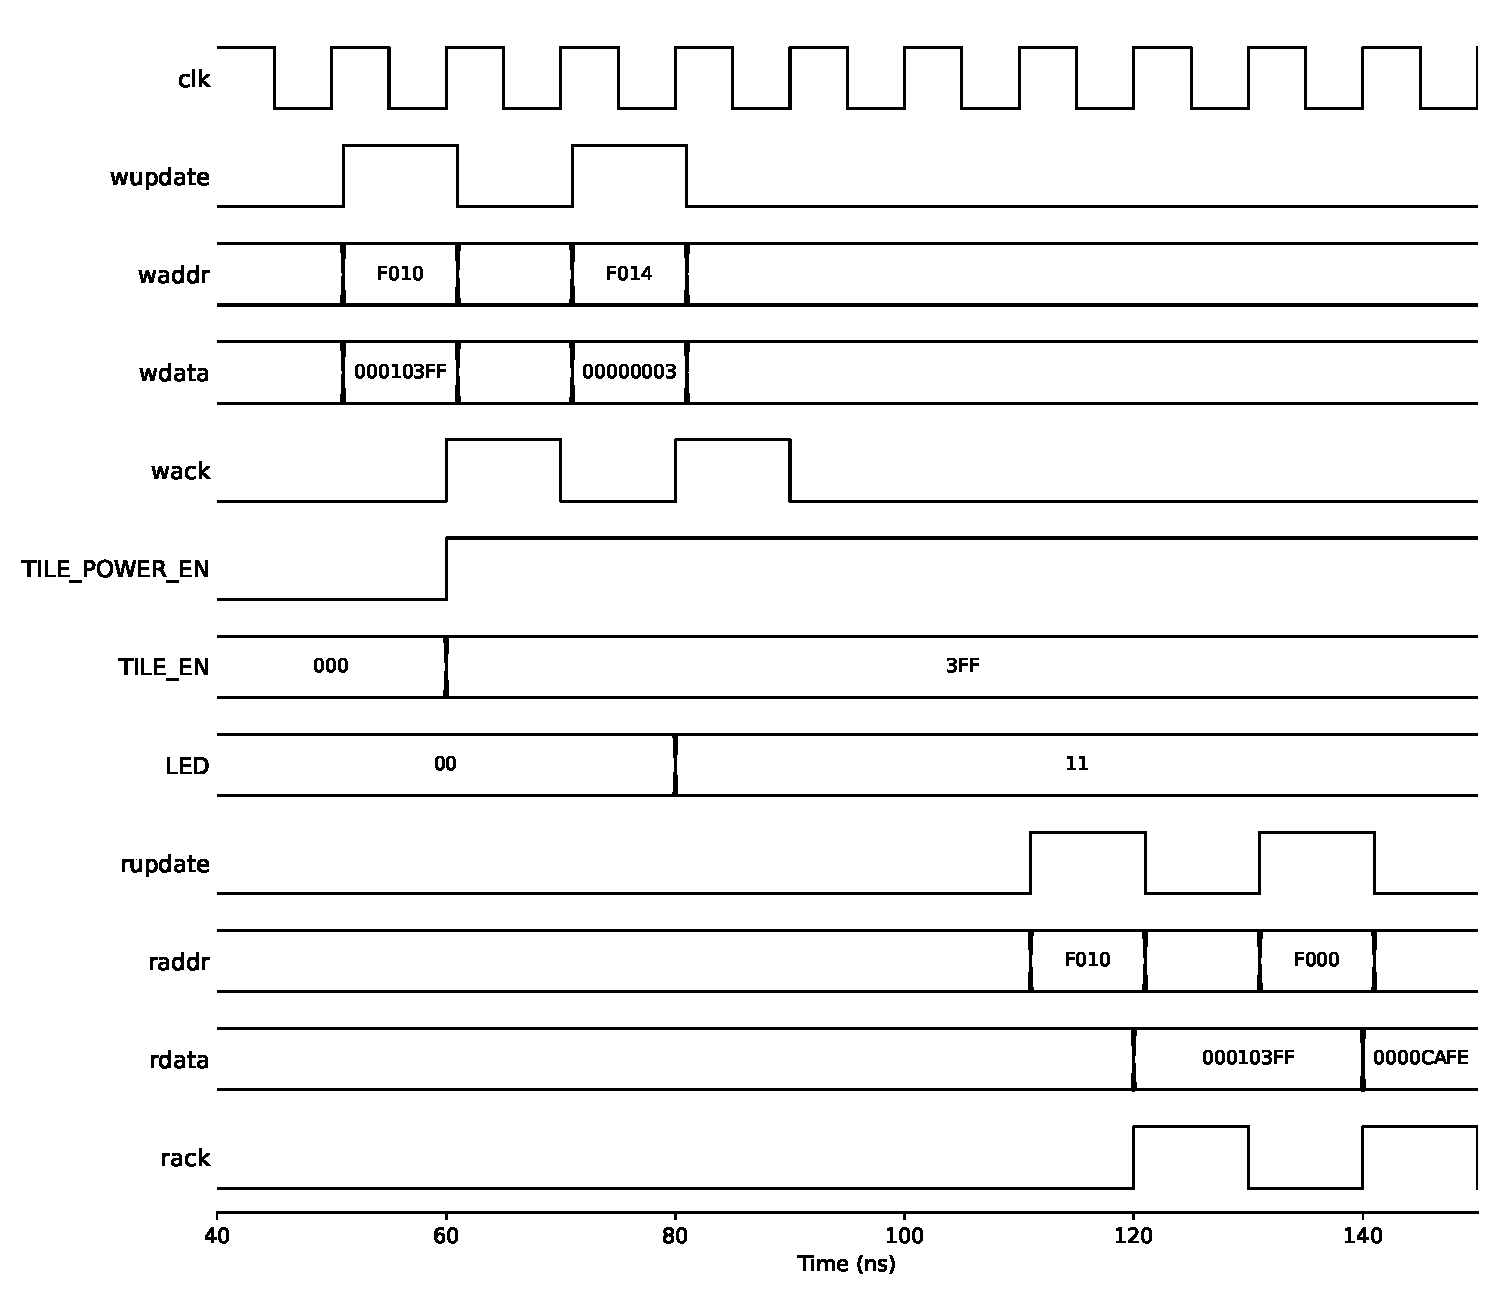
\includegraphics[width=0.9\textwidth]{figs/global.pdf}
  \caption{\label{fig:global} The Global unit on the register bus (GHDL simulation of {\tt global\_unit}).
    Two writes, ENABLES (\hex{F010}) with tile power and all ten tiles, and LEDS (\hex{F014}) with both
    LEDs on, each acknowledged on the next clock cycle, at which time the outputs change.  Then reads of
    ENABLES and STATUS, each answered on the next clock cycle.}
\end{figure}

The Global unit handles simple board-wide tasks, through the registers of Table~\ref{tbl:global-reg}.

\begin{table}[htbp]
\caption{\label{tbl:global-reg} Registers of the Global unit.}
\begin{center}\small
\begin{tabularx}{\textwidth}{llcL}
\toprule
Register          & Address     & Access & Contents \\
\midrule
STATUS            & \hex{F000} & RO & fixed pattern \hex{0000CAFE} \\
ENABLES           & \hex{F010} & RW & tile enables and tile power (Table~\ref{tbl:global-bits}) \\
LEDS              & \hex{F014} & RW & the two LEDs driven by the PL (Table~\ref{tbl:global-bits}) \\
SCRATCH\_A        & \hex{F020} & RW & no effect: for testing the register path \\
SCRATCH\_B        & \hex{F024} & RW & no effect: for testing the register path \\
FIRMWARE\_MAJOR   & \hex{FF10} & RO & firmware version: 3 \\
FIRMWARE\_MINOR   & \hex{FF14} & RO & firmware version: 6 \\
FIRMWARE\_PATCH   & \hex{FF18} & RO & firmware version: 0 \\
HARDWARE\_MAJOR   & \hex{FF20} & RO & hardware version the firmware was built for: 1 \\
HARDWARE\_MINOR   & \hex{FF24} & RO & hardware version: 5 \\
HARDWARE\_PATCH   & \hex{FF28} & RO & hardware version: 0 \\
SYNTHESIS\_DATE   & \hex{FF30} & RO & time of the build, in seconds since 1970 (Unix time) \\
GIT\_HASH\_UPPER  & \hex{FF40} & RO & short git hash of the build, ASCII, characters 1--4 \\
GIT\_HASH\_LOWER  & \hex{FF44} & RO & short git hash, ASCII, characters 5--7 and a space \\
BUILD\_FLAGS      & \hex{FF48} & RO & bit 0 DIRTY, bit 1 OFFICIAL\_RELEASE \\
VIVADO\_MAJOR     & \hex{FF50} & RO & Vivado version of the build (e.g.\ 2023) \\
VIVADO\_MINOR     & \hex{FF54} & RO & Vivado version of the build (e.g.\ 2) \\
\bottomrule
\end{tabularx}
\end{center}
\end{table}

\begin{table}[htbp]
\caption{\label{tbl:global-bits} Bit fields of the Global registers.}
\begin{center}
\begin{tabular}{llll}
\toprule
Register & Field               & Bits  & Mask \\
\midrule
ENABLES  & TILE\_ENABLES       & 9--0  & \hex{000003FF} \\
         & TILE\_POWER\_ENABLE & 16    & \hex{00010000} \\
\midrule
LEDS     & LED\_3              & 0     & \hex{00000001} \\
         & LED\_4              & 1     & \hex{00000002} \\
\bottomrule
\end{tabular}
\end{center}
\end{table}

Powering a tile requires enabling the tile power subsystem with TILE\_POWER\_ENABLE (called
ANALOG\_POWER\_ENABLE in the schematics) as well as the tile itself, with its bit of TILE\_ENABLES.  The
other bits of ENABLES, and bits 31--2 of LEDS, are stored and read back, but drive nothing.  Each of the two
PL LEDs is simply on or off, as set by its bit of LEDS; the two other LEDs of the PACMAN are driven by the PS.
Voltages, currents and the on-board multiplexer are controlled over I2C by the PS, and are not part of the
PL.

The version registers identify the firmware without reference to any file.  The firmware and hardware
versions are constants of the source ({\tt firmware\_version.vhd}, {\tt hardware\_version.vhd}).  The
synthesis date, git hash, build flags and Vivado version are written at build time.  DIRTY is set when the
Vivado sources ({\tt vivado/}) had uncommitted changes at the time of the build; OFFICIAL\_RELEASE is set when
the build was made from a commit marked as an official release (with the {\tt BUILD\_RELEASE} file).  In a GHDL simulation these build-time registers all
read zero.

As in Fig.~\ref{fig:global}, the Global unit acknowledges reads and writes on the next clock cycle, and a
register written is visible at its output from that same clock cycle.

%======================================================================
\section{TX unit}

\begin{figure}[htbp]
\centering
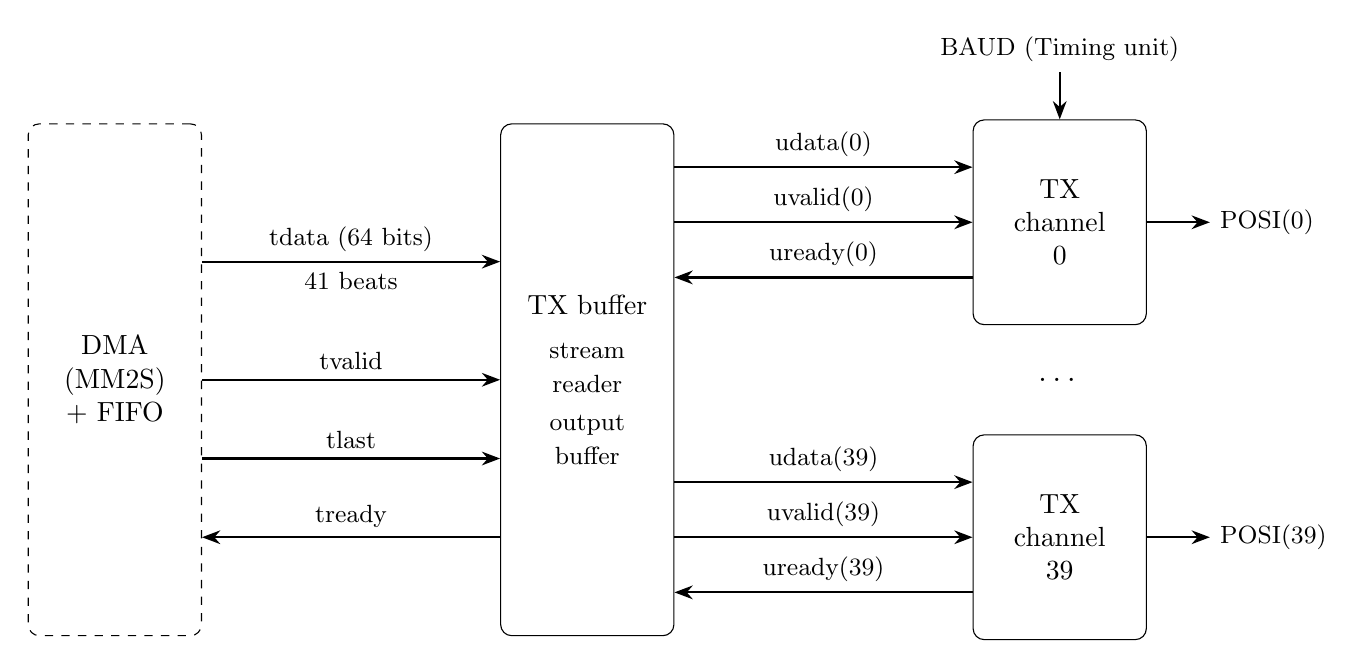
\begin{tikzpicture}[x=1cm, y=1cm, >=Stealth]
\def\bw{2.2cm}
\node[draw, rounded corners, dashed, minimum width=\bw, minimum height=6.5cm, align=center] (dma) at (0,3) {DMA\\(MM2S)\\+ FIFO};
\node[draw, rounded corners, minimum width=\bw, minimum height=6.5cm, align=center] (buf) at (6,3) {TX buffer\\[4pt]\small stream\\\small reader\\[2pt]\small output\\\small buffer};
\node[draw, rounded corners, minimum width=\bw, minimum height=2.6cm, align=center] (a) at (12,5) {TX\\channel\\0};
\node[draw, rounded corners, minimum width=\bw, minimum height=2.6cm, align=center] (b) at (12,1) {TX\\channel\\39};
\node at (12,3) {\large\textellipsis};
\draw[->, thick] ($(dma.east)+(0,1.5)$) -- node[above, font=\small] {tdata (64 bits)} node[below, font=\small] {41 beats} ($(buf.west)+(0,1.5)$);
\draw[->, thick] ($(dma.east)+(0,0)$) -- node[above, font=\small] {tvalid} ($(buf.west)+(0,0)$);
\draw[->, thick] ($(dma.east)-(0,1)$) -- node[above, font=\small] {tlast} ($(buf.west)-(0,1)$);
\draw[<-, thick] ($(dma.east)-(0,2)$) -- node[above, font=\small] {tready} ($(buf.west)-(0,2)$);
\foreach \n/\k in {a/0, b/39} {
  \draw[->, thick] (buf.east |- {$(\n.west)+(0,0.7)$}) -- node[above, font=\small] {udata(\k)} ($(\n.west)+(0,0.7)$);
  \draw[->, thick] (buf.east |- \n.west) -- node[above, font=\small] {uvalid(\k)} (\n.west);
  \draw[<-, thick] (buf.east |- {$(\n.west)-(0,0.7)$}) -- node[above, font=\small] {uready(\k)} ($(\n.west)-(0,0.7)$);
  \draw[->, thick] (\n.east) -- ++(0.8,0) node[anchor=west, font=\small] {POSI(\k)};
}
\draw[<-, thick] ($(a.north)$) -- ++(0,0.6) node[anchor=south, font=\small] {BAUD (Timing unit)};
\end{tikzpicture}
\caption{\label{fig:tx-unit} Data path of the TX unit.}
\end{figure}

The TX unit transmits data from the PS to the tiles over 40 UART channels.  Its data path is shown in
Fig.~\ref{fig:tx-unit}.  The PS fills a DMA packet in memory; the DMA engine streams it to the TX buffer
(through a FIFO that crosses into the TX unit's clock domain); the TX buffer hands each UART its 64-bit
word; and 40 TX channels, one per UART, transmit their words in parallel on the POSI lines.

\subsection{DMA packet}

\begin{table}[htbp]
\caption{\label{tbl:tx-dma} The TX DMA packet: 41 beats of 64 bits, TLAST on the last.}
\begin{center}
\begin{tabular}{lll}
\toprule
Beat & Contents (64 bits)                    & Description \\
\midrule
0    & \texttt{0x000000MMMMMMMMMM}           & M: UART mask, bit $i$ for UART $i$ \\
1    & \texttt{0xDDDDDDDDDDDDDDDD}           & D: the word for UART 0 \\
2    & \texttt{0xDDDDDDDDDDDDDDDD}           & the word for UART 1 \\
     & \ldots                                & \\
40   & \texttt{0xDDDDDDDDDDDDDDDD}           & the word for UART 39 \\
\bottomrule
\end{tabular}
\end{center}
\end{table}

A DMA packet is always 41 beats of 64 bits (328 bytes), as in Table~\ref{tbl:tx-dma}: a mask with one bit per
UART, then one 64-bit word per UART, in UART order.  Only the UARTs selected by the mask transmit; the words
of the others are ignored.  The packet is the same size however many UARTs are selected.  The length is not
checked by the firmware: a packet that ends early (TLAST before beat 40) leaves the missing words as they
were in the previous packet.

\subsection{TX buffer}

\begin{figure}[htbp]
  \centering
  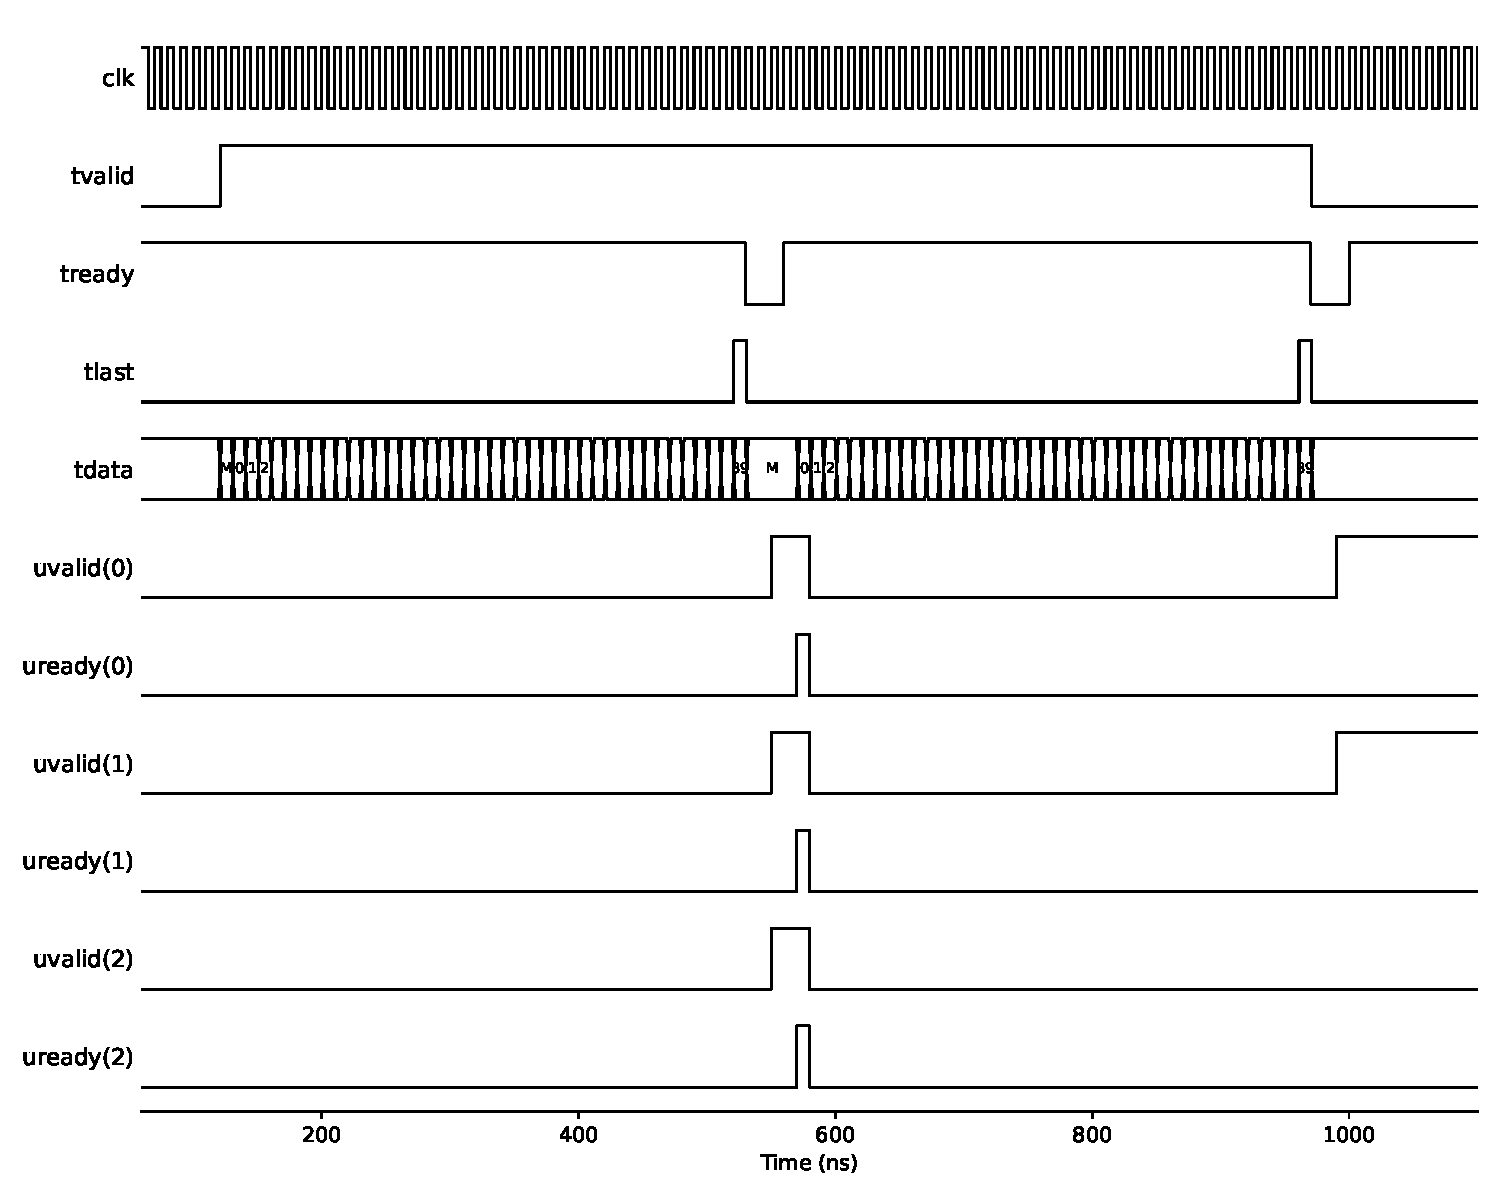
\includegraphics[width=0.9\textwidth]{figs/tx_stream.pdf}
  \caption{\label{fig:tx-stream} The TX buffer receiving two DMA packets back to back (GHDL simulation of
    {\tt tx\_unit}).  Packet 1 selects UARTs 0--2, packet 2 UARTs 0 and 1.  On tdata, M is the mask beat and
    the numbers are the UART of each word (labels shown for UARTs 0--2 and 39 only).  The TX buffer drops
    tready for three clock cycles after each packet, while the packet moves to the output buffer.  The
    channels of packet 1 take their words at once (uready); those of packet 2 are still transmitting packet
    1, so the words of packet 2 wait in the output buffer (uvalid stays high, beyond the end of the figure).}
\end{figure}

The TX buffer has two stages.  The first, the stream reader, collects the 41 beats of a packet.  Once a
complete packet has arrived (TLAST), it deasserts tready, and the packet is copied into the second stage, the
output buffer: one 64-bit word per UART, with a valid bit (uvalid) set for each UART of the mask.  The
stream reader is then released and asserts tready again, ready for the next packet, while the UARTs
transmit.  The whole hand-over takes three clock cycles (Fig.~\ref{fig:tx-stream}).

Each TX channel takes its word when it is ready to start a new transmission: it asserts uready for one clock
cycle, which clears that UART's uvalid on the next clock cycle.  The output buffer accepts the next packet
only when every uvalid bit is clear, that is, when every selected UART has taken its word.  With the UART
shift registers, the output buffer and the stream reader, up to three packets are in the TX unit at once:
one being transmitted, one waiting in the output buffer, and one waiting in the stream reader, as in
Fig.~\ref{fig:tx-stream}.

The UART transmission is by far the slowest step.  At the default bit rate of 10 Mbit/s, a 66-bit frame (a
start bit, 64 data bits and a stop bit) takes 6.6\,$\mu$s, or 660 clock cycles; a DMA packet takes 41 clock
cycles.  As long as DMA keeps the stream reader full, the TX channels transmit back to back, separated only
by their configured delay.

\subsection{TX channel}

\begin{figure}[htbp]
  \centering
  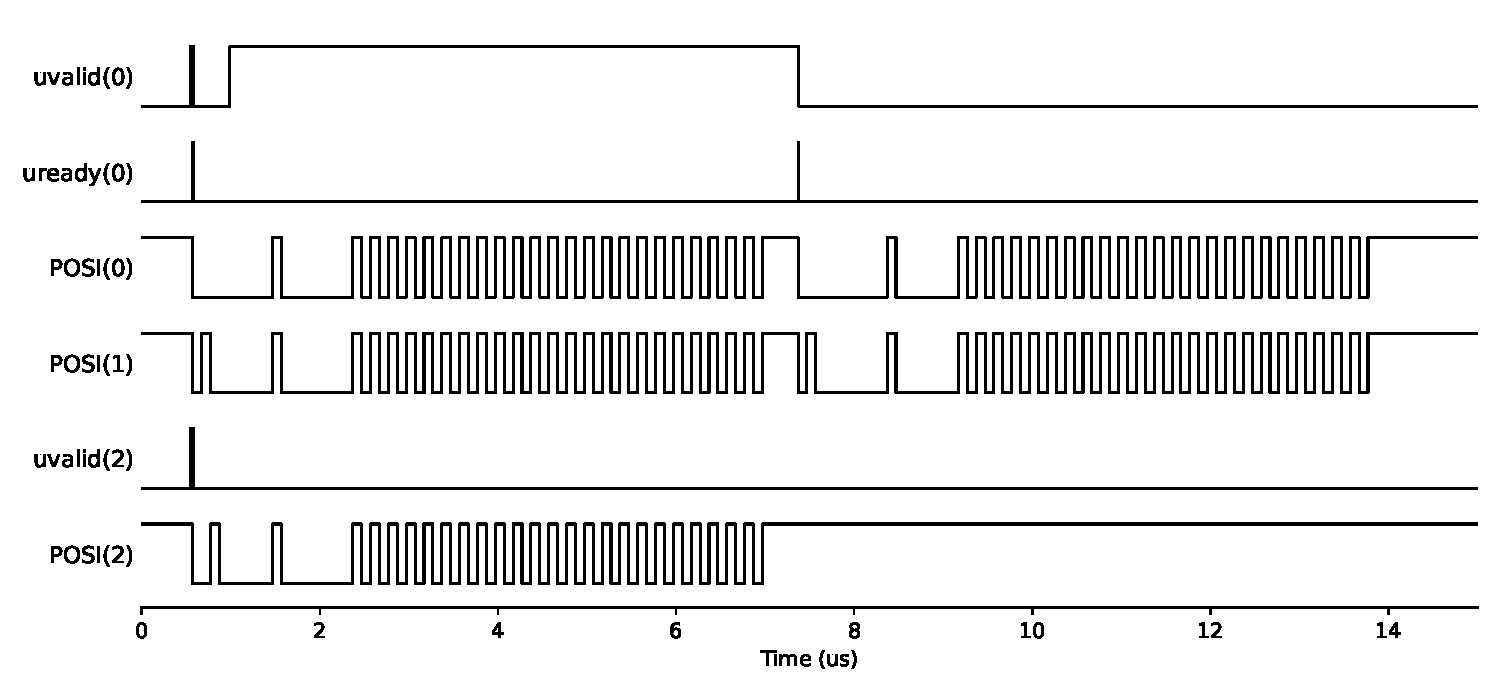
\includegraphics[width=0.9\textwidth]{figs/tx_frames.pdf}
  \caption{\label{fig:tx-frames} The UART frames of the two packets of Fig.~\ref{fig:tx-stream} (GHDL
    simulation of {\tt tx\_unit}; all UARTs configured \hex{00020006}: PHASE 6, DELAY 2).  Each word is
    \hex{AAAAAAAAAAAA} above a 16-bit identifier ({\tt 0x0n0u}: packet $n$, UART $u$), sent least
    significant bit first, so each frame shows a start bit, 16 identifier bits, then 48 alternating bits,
    and a stop bit.  UARTs 0 and 1 take the second word (uready) after the stop bit and the 2-bit delay.}
\end{figure}

Each TX channel is a UART transmitter with a 64-bit shift register.  Its bit timing comes from the BAUD
strobe of the Timing unit, one clock cycle at the start of each bit period (every 10 clock cycles, or
10 Mbit/s, by default).  The channel acts PHASE clock cycles after each BAUD strobe; PHASE sets the position
of the bit edges within the bit period, and is the same for all channels unless configured otherwise.

While idle, the line is high.  At the first bit boundary at which valid data is offered (uvalid), the channel
loads the word, asserts uready for one clock cycle, and sends the start bit (low).  It then sends the 64 data
bits, least significant first, then the stop bit (high).  It then waits DELAY further bit periods, with the
line high, before it may load the next word.  With DELAY = 0, frames follow each other with no gap: 66 bit
periods per word.  DELAY throttles the transmission rate, to avoid overwhelming the ASICs.

Figure~\ref{fig:tx-frames} shows the frames of the two packets of Fig.~\ref{fig:tx-stream}.  UART 2, selected
only in packet 1, sends one frame; UARTs 0 and 1 send their second word directly after the stop bit and the
delay of the first.

\subsection{TX registers}

\begin{table}[htbp]
\caption{\label{tbl:tx-reg} Registers of the TX unit (scope \texttt{00}).  Per UART registers are at channel
  0--39 (\hex{00}--\hex{27}); UART\_CONFIG can also be written at the broadcast channel (\hex{3B}).  Common
  registers are at channel \hex{3F}.  $R$ is the register byte of the address.}
\begin{center}\small
\begin{tabularx}{\textwidth}{lllcL}
\toprule
Register        & $R$        & Channel  & Access & Contents \\
\midrule
UART\_STATUS    & \hex{00} & UART & RO  & channel status (Table~\ref{tbl:tx-bits}) \\
UART\_CONFIG    & \hex{04} & UART & RW & PHASE and DELAY (Table~\ref{tbl:tx-bits}); default \hex{00000006} \\
UART\_STARTS    & \hex{20} & UART & RO  & counter: frames started (start bits sent) \\
UART\_BEATS     & \hex{24} & UART & RO  & counter: words taken from the TX buffer (uvalid and uready) \\
LOOK\_SELECT    & \hex{A0} & common   & RW  & the UART shown by LOOK\_UA and LOOK\_UB \\
LOOK\_UA        & \hex{A4} & common   & RO  & that UART's word in the output buffer, bits 31--0 \\
LOOK\_UB        & \hex{A8} & common   & RO  & that UART's word in the output buffer, bits 63--32 \\
BUFFER\_STATUS  & \hex{B0} & common   & RO  & TX buffer status (Table~\ref{tbl:tx-bits}) \\
ZERO\_CNTS      & \hex{F8} & common   & WO  & clear all TX counters (command: any value) \\
\bottomrule
\end{tabularx}
\end{center}
\end{table}

\begin{table}[htbp]
\caption{\label{tbl:tx-bits} Bit fields of the TX registers.}
\begin{center}\small
\begin{tabularx}{\textwidth}{lllL}
\toprule
Register       & Field   & Bits   & Description \\
\midrule
UART\_CONFIG   & PHASE   & 7--0   & clock cycles from the BAUD strobe to the bit edges \\
               & DELAY   & 31--16 & bit periods of idle line between frames \\
\midrule
UART\_STATUS   & START   & 0      & a start bit was sent (one clock cycle) \\
               & TX      & 1      & the POSI line \\
               & VALID   & 2      & uvalid (a word is waiting for this UART) \\
               & READY   & 3      & uready (the word is taken; one clock cycle) \\
               & STATE   & 5--4   & 0 idle, 1 shifting, 2 stop bit, 3 delay \\
               & BIT     & 6      & the bit-edge strobe (BAUD + PHASE) \\
\midrule
BUFFER\_STATUS & TREADY  & 0      & stream tready \\
               & TVALID  & 1      & stream tvalid \\
               & RELEASE & 4      & the stream reader is released (one clock cycle) \\
               & PACKET  & 5      & the stream reader holds a complete packet \\
               & STATE   & 9--8   & 0 idle, 1 start of transmission, 2 transmitting \\
\bottomrule
\end{tabularx}
\end{center}
\end{table}

The registers of the TX unit are listed in Table~\ref{tbl:tx-reg}, and their bit fields in
Table~\ref{tbl:tx-bits}.  The configuration of each UART (UART\_CONFIG) holds PHASE and DELAY; the bit
period itself is set for all UARTs by the Timing unit (CONFIG\_BAUD).  The counters count, for each UART, the
frames started (UART\_STARTS) and the words taken from the TX buffer (UART\_BEATS); the two are equal in
normal operation.  The look registers show the word waiting in, or last loaded from, the output buffer for one
UART: they check the path from DMA to the TX buffer, not the UART transmitter itself, which can be checked
by the RX loopback (Section~\ref{sec:rx-chan}).  The status registers are snapshots, mainly useful for
debugging.

%======================================================================
\section{RX unit}

\begin{figure}[htbp]
\centering
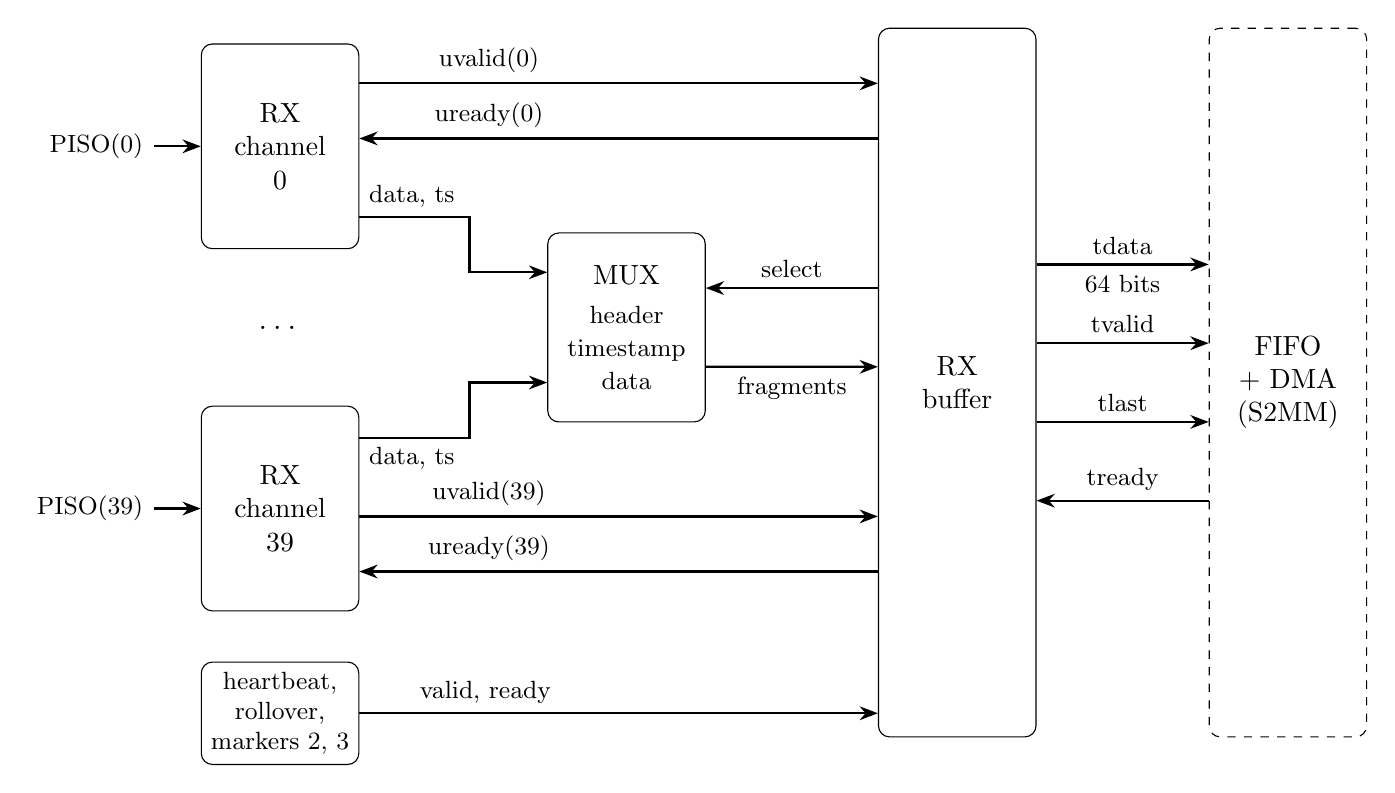
\begin{tikzpicture}[x=1cm, y=1cm, >=Stealth]
\def\bw{2.0cm}
\node[draw, rounded corners, minimum width=\bw, minimum height=2.6cm, align=center] (a) at (0,5.6) {RX\\channel\\0};
\node[draw, rounded corners, minimum width=\bw, minimum height=2.6cm, align=center] (b) at (0,1.0) {RX\\channel\\39};
\node at (0,3.3) {\large\textellipsis};
\node[draw, rounded corners, minimum width=\bw, minimum height=1.3cm, align=center, font=\small] (x) at (0,-1.6) {heartbeat,\\rollover,\\markers 2, 3};
\node[draw, rounded corners, minimum width=\bw, minimum height=2.4cm, align=center] (mux) at (4.4,3.3) {MUX\\[2pt]\small header\\\small timestamp\\\small data};
\node[draw, rounded corners, minimum width=\bw, minimum height=9.0cm, align=center] (buf) at (8.6,2.6) {RX\\buffer};
\node[draw, rounded corners, dashed, minimum width=\bw, minimum height=9.0cm, align=center] (fifo) at (12.8,2.6) {FIFO\\+ DMA\\(S2MM)};
% UART 0:  valid and ready above the mux, data and timestamp into the mux
\draw[->, thick] ($(a.east)+(0,0.8)$) -- node[above, font=\small, pos=0.25] {uvalid(0)} (buf.west |- {$(a.east)+(0,0.8)$});
\draw[<-, thick] ($(a.east)+(0,0.1)$) -- node[above, font=\small, pos=0.25] {uready(0)} (buf.west |- {$(a.east)+(0,0.1)$});
\draw[->, thick] ($(a.east)-(0,0.9)$) -- ++(1.4,0) |- ($(mux.west)+(0,0.7)$);
\node[font=\small, anchor=south west] at ($(a.east)-(0,0.9)$) {data, ts};
% UART 39:  data and timestamp into the mux, valid and ready below it
\draw[->, thick] ($(b.east)+(0,0.9)$) -- ++(1.4,0) |- ($(mux.west)-(0,0.7)$);
\node[font=\small, anchor=north west] at ($(b.east)+(0,0.9)$) {data, ts};
\draw[->, thick] ($(b.east)-(0,0.1)$) -- node[above, font=\small, pos=0.25] {uvalid(39)} (buf.west |- {$(b.east)-(0,0.1)$});
\draw[<-, thick] ($(b.east)-(0,0.8)$) -- node[above, font=\small, pos=0.25] {uready(39)} (buf.west |- {$(b.east)-(0,0.8)$});
% the extra channels
\draw[->, thick] (x.east) -- (buf.west |- x.east);
\node[font=\small, anchor=south] at ($(x.east)+(1.6,0)$) {valid, ready};
\foreach \n/\k in {a/0, b/39} \draw[<-, thick] (\n.west) -- ++(-0.6,0) node[anchor=east, font=\small] {PISO(\k)};
% mux and buffer
\draw[<-, thick] ($(mux.east)+(0,0.5)$) -- node[above, font=\small] {select} ($(buf.west)+(0,1.2)$);
\draw[->, thick] ($(mux.east)-(0,0.5)$) -- node[below, font=\small] {fragments} ($(buf.west)-(0,0.5)+(0,0.7)$);
% stream
\draw[->, thick] ($(buf.east)+(0,1.5)$) -- node[above, font=\small] {tdata} node[below, font=\small] {64 bits} ($(fifo.west)+(0,1.5)$);
\draw[->, thick] ($(buf.east)+(0,0.5)$) -- node[above, font=\small] {tvalid} ($(fifo.west)+(0,0.5)$);
\draw[->, thick] ($(buf.east)-(0,0.5)$) -- node[above, font=\small] {tlast} ($(fifo.west)-(0,0.5)$);
\draw[<-, thick] ($(buf.east)-(0,1.5)$) -- node[above, font=\small] {tready} ($(fifo.west)-(0,1.5)$);
\end{tikzpicture}
\caption{\label{fig:rx-unit} Data path of the RX unit.  Each RX channel presents its word (data and
  timestamp) with a valid bit.  The RX buffer selects one channel at a time; the multiplexer presents that
  channel's three 64-bit fragments (header, timestamp, data), which the buffer writes to the stream.  The
  heartbeat, rollover and marker sources are four further channels (their timestamps also pass the
  multiplexer).}
\end{figure}

The RX unit receives the UART words from the tiles and streams them to the PS.  Its data path is shown in
Fig.~\ref{fig:rx-unit}.  Forty RX channels receive the PISO lines independently.  Each completed word is
held, with its timestamp, until the RX buffer takes it.  The RX buffer visits the channels in turn and writes
each waiting word to the AXI stream, as a 192-bit stream word of three 64-bit fragments: a header, the
timestamp, and the data.  It closes the stream into DMA packets (TLAST).  An AXI stream FIFO crosses into the
PS clock domain, and the DMA engine writes the packets to memory.

\subsection{RX channel}\label{sec:rx-chan}

\begin{figure}[htbp]
  \centering
  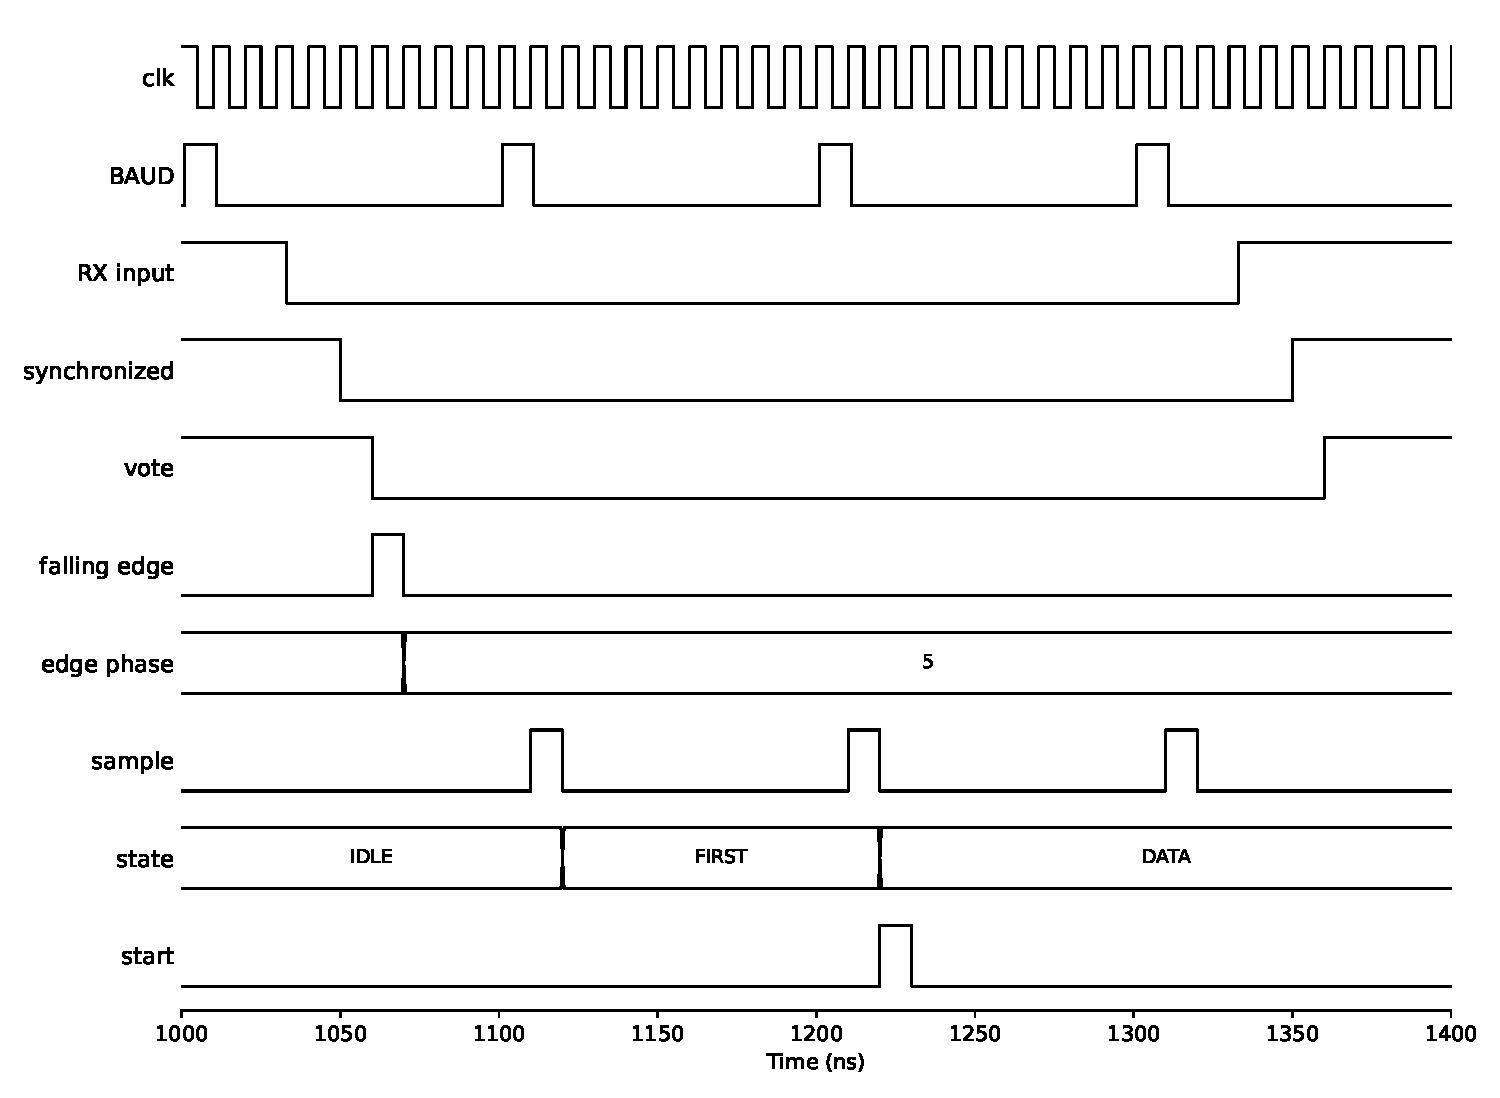
\includegraphics[width=0.9\textwidth]{figs/rx_chan_start.pdf}
  \caption{\label{fig:rx-chan-start} An RX channel finding the start bit (GHDL simulation of {\tt rx\_chan};
    default configuration \hex{000A1104}: PERIOD 10, MODE 1, INPUT 1, PHASE 4; BAUD every 10 clock cycles).
    The input falls at 1033\,ns, asynchronously to the clock.  After the two-stage synchronizer and the
    three-sample history, the falling edge is detected five clock cycles after the BAUD strobe (edge phase
    5).  The sample point is set PHASE = 4 clock cycles after the edge phase, in every bit period: the first
    sample sees the start bit (state FIRST), the next one data bit 0, where the start flag is raised, and
    every following sample one more data bit.}
\end{figure}

Each RX channel is a UART receiver with a 64-bit shift register.  The input is chosen by the INPUT field of
the channel's configuration: the PISO line from the tile (normal operation), the channel's own TX output
(POSI, a loopback through the PL only), the RX test pattern (Section~\ref{sec:rx-pattern}), or none (the line
held high).  The selected input is asynchronous to the PL clock.  It passes a two-stage synchronizer, and
then a three-sample history, which gives a majority vote of the last three samples, a flag when they
disagree (dissent), and a glitch-free falling-edge detection (two low samples after a high one).

The receiver samples the line once per bit period.  In the normal mode (MODE 1), the sample point follows the
start bit: while the channel is idle, the falling edge of a start bit is located within the bit period (the
number of clock cycles since the last BAUD strobe, the {\em edge phase}), and the sample point is set PHASE
clock cycles later, modulo PERIOD.  PERIOD must equal the bit period set in the Timing unit (CONFIG\_BAUD;
10 by default).  The default PHASE of 4 puts the sample near the middle of the bit, allowing for the delay of
the synchronizer.  In the fixed mode (MODE 2), the sample point is PHASE clock cycles after each BAUD strobe,
whatever the input.  With MODE 0 the channel never samples, so it receives nothing.

At each sample point the majority vote is taken.  A low vote while idle is a start bit: the following 64
samples are the data bits, least significant first, and the next sample is the stop bit
(Fig.~\ref{fig:rx-chan-start}).  A start bit is accepted only if its three samples agree, unless flag bit 14
of the configuration is set.  A sample at which the three samples disagree is counted as noise.

\begin{figure}[htbp]
  \centering
  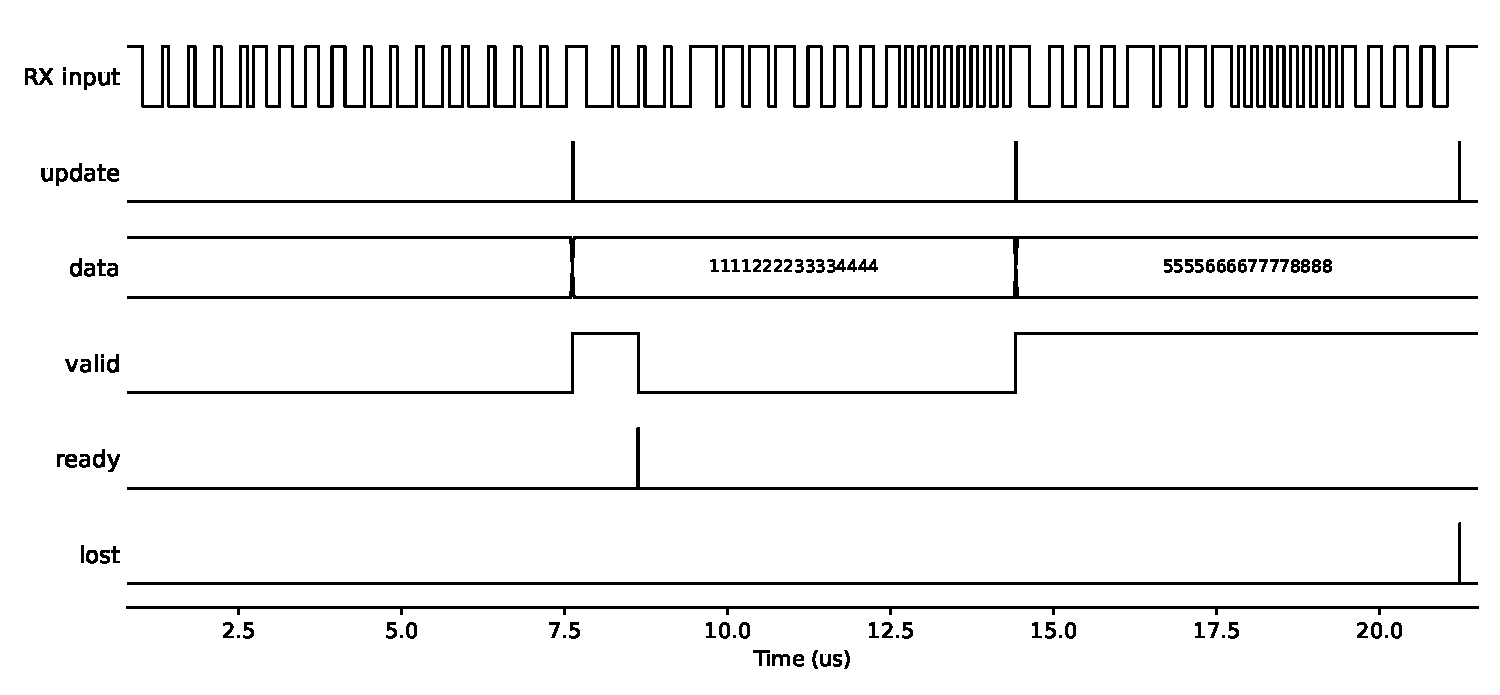
\includegraphics[width=0.9\textwidth]{figs/rx_chan_frames.pdf}
  \caption{\label{fig:rx-chan-frames} An RX channel receiving three frames back to back (same simulation as
    Fig.~\ref{fig:rx-chan-start}).  The first word is taken by the RX buffer (ready) soon after it is valid;
    the second is held, valid, since it is not taken; the third arrives while the second is still valid, and
    is lost.}
\end{figure}

A high stop bit completes the frame (update): the word is copied to the channel's output, together with the
timestamp of the Timing unit at that moment, and the channel asserts valid.  Valid is cleared when the RX
buffer takes the word (ready).  The output holds one word only: if a further frame completes while valid is
still set, the new word is discarded and counted as lost (Fig.~\ref{fig:rx-chan-frames}).  A low stop bit is a
framing error: the word is discarded and counted.  In normal operation the RX buffer takes each word within one sweep
of its channels (135 clock cycles, Section~\ref{sec:rx-buffer}), far less than the 660 clock cycles of a
frame, so no word is lost.

\subsection{Stream words}

\begin{table}[htbp]
\caption{\label{tbl:rx-word} An RX stream word: three 64-bit fragments.  For the extra channels (40--43)
  the header is the HEADER\_A--D register with the PACMAN identifier in bits 15--8, and the data fragment is
  zero.}
\begin{center}
\begin{tabularx}{\textwidth}{llL}
\toprule
Fragment   & Bits    & Contents \\
\midrule
header     & 7--0    & word type: WORD\_TYPE\_LUT byte chosen by the two least significant data bits \\
           & 15--8   & PACMAN identifier (PACMAN register, bits 7--0) \\
           & 31--16  & channel identifier (UART\_CHAN register of the UART; default UART number + 1) \\
           & 63--32  & zero \\
timestamp  & 63--0   & timestamp at the completion of the word (Timing unit) \\
data       & 63--0   & the received UART word \\
\bottomrule
\end{tabularx}
\end{center}
\end{table}

\begin{table}[htbp]
\caption{\label{tbl:rx-chan} The 44 channels of the RX buffer, visited in this order.  The extra channels
  are each enabled by one bit of BUFFER\_ENABLES (all off by default).}
\begin{center}
\begin{tabularx}{\textwidth}{llLl}
\toprule
Turn   & Source          & Header (default)                 & Enable \\
\midrule
0--39  & UART 0--39      & channel id, PACMAN id, word type & always \\
40     & heartbeat       & HEADER\_A (\hex{00480053}, type `S') & BUFFER\_ENABLES bit 0 \\
41     & rollover        & HEADER\_B (\hex{00530053}, type `S') & BUFFER\_ENABLES bit 1 \\
42     & marker 2        & HEADER\_C (\hex{00000054}, type `T') & BUFFER\_ENABLES bit 2 \\
43     & marker 3        & HEADER\_D (\hex{00000000})       & BUFFER\_ENABLES bit 3 \\
\midrule
trailer & end of packet  & EOP\_HEADER (\hex{0000004C}, type `L'), then the word count, then zero & \\
\bottomrule
\end{tabularx}
\end{center}
\end{table}

Each word in the stream is 192 bits, sent as three 64-bit fragments (Table~\ref{tbl:rx-word}).  The header
identifies the word.  Its word type is one byte of the WORD\_TYPE\_LUT register, chosen by the two least
significant bits of the data (for LArPix, the packet type); by default all four bytes are \hex{44}, the
character `D'.  The PACMAN identifier is set by the PACMAN register, and the channel identifier of each UART by
its UART\_CHAN register, so that the PS can label the data without further bookkeeping.

Besides the 40 UARTs, the RX buffer serves four extra channels (Table~\ref{tbl:rx-chan}), each of which adds
a word with a timestamp to the stream:
\begin{itemize}
\item {\bf heartbeat} (channel 40): a word every HEARTBEAT\_CONFIG clock cycles (default \hex{3B9ACA00}, $10^9$
  clock cycles: every 10\,s).  A heartbeat that is not yet taken delays the next one; none is lost.
\item {\bf rollover} (channel 41): a word each time the least significant 32 bits of the timestamp equal
  ROLLOVER\_CONFIG.  The default, 1, marks each wrap of the 32-bit timestamp: once every $2^{32}$ periods of
  the ASIC clock, about 7.2 minutes at 10 MHz.
\item {\bf markers 2 and 3} (channels 42 and 43): a word for each pulse of marker 2 or 3 of the Timing unit
  (Section~\ref{sec:atc}), for instance for a LEMO trigger input.
\end{itemize}
The header of an extra-channel word is the register HEADER\_A to HEADER\_D, with bits 15--8 replaced by the
PACMAN identifier, and its data fragment is zero.  The packet trailer (below) is a word too: its header is
EOP\_HEADER, also with the PACMAN identifier in bits 15--8, its second fragment the number of
words in the packet (not counting the trailer), and its third fragment zero.

\subsection{RX buffer}\label{sec:rx-buffer}

\begin{figure}[htbp]
  \centering
  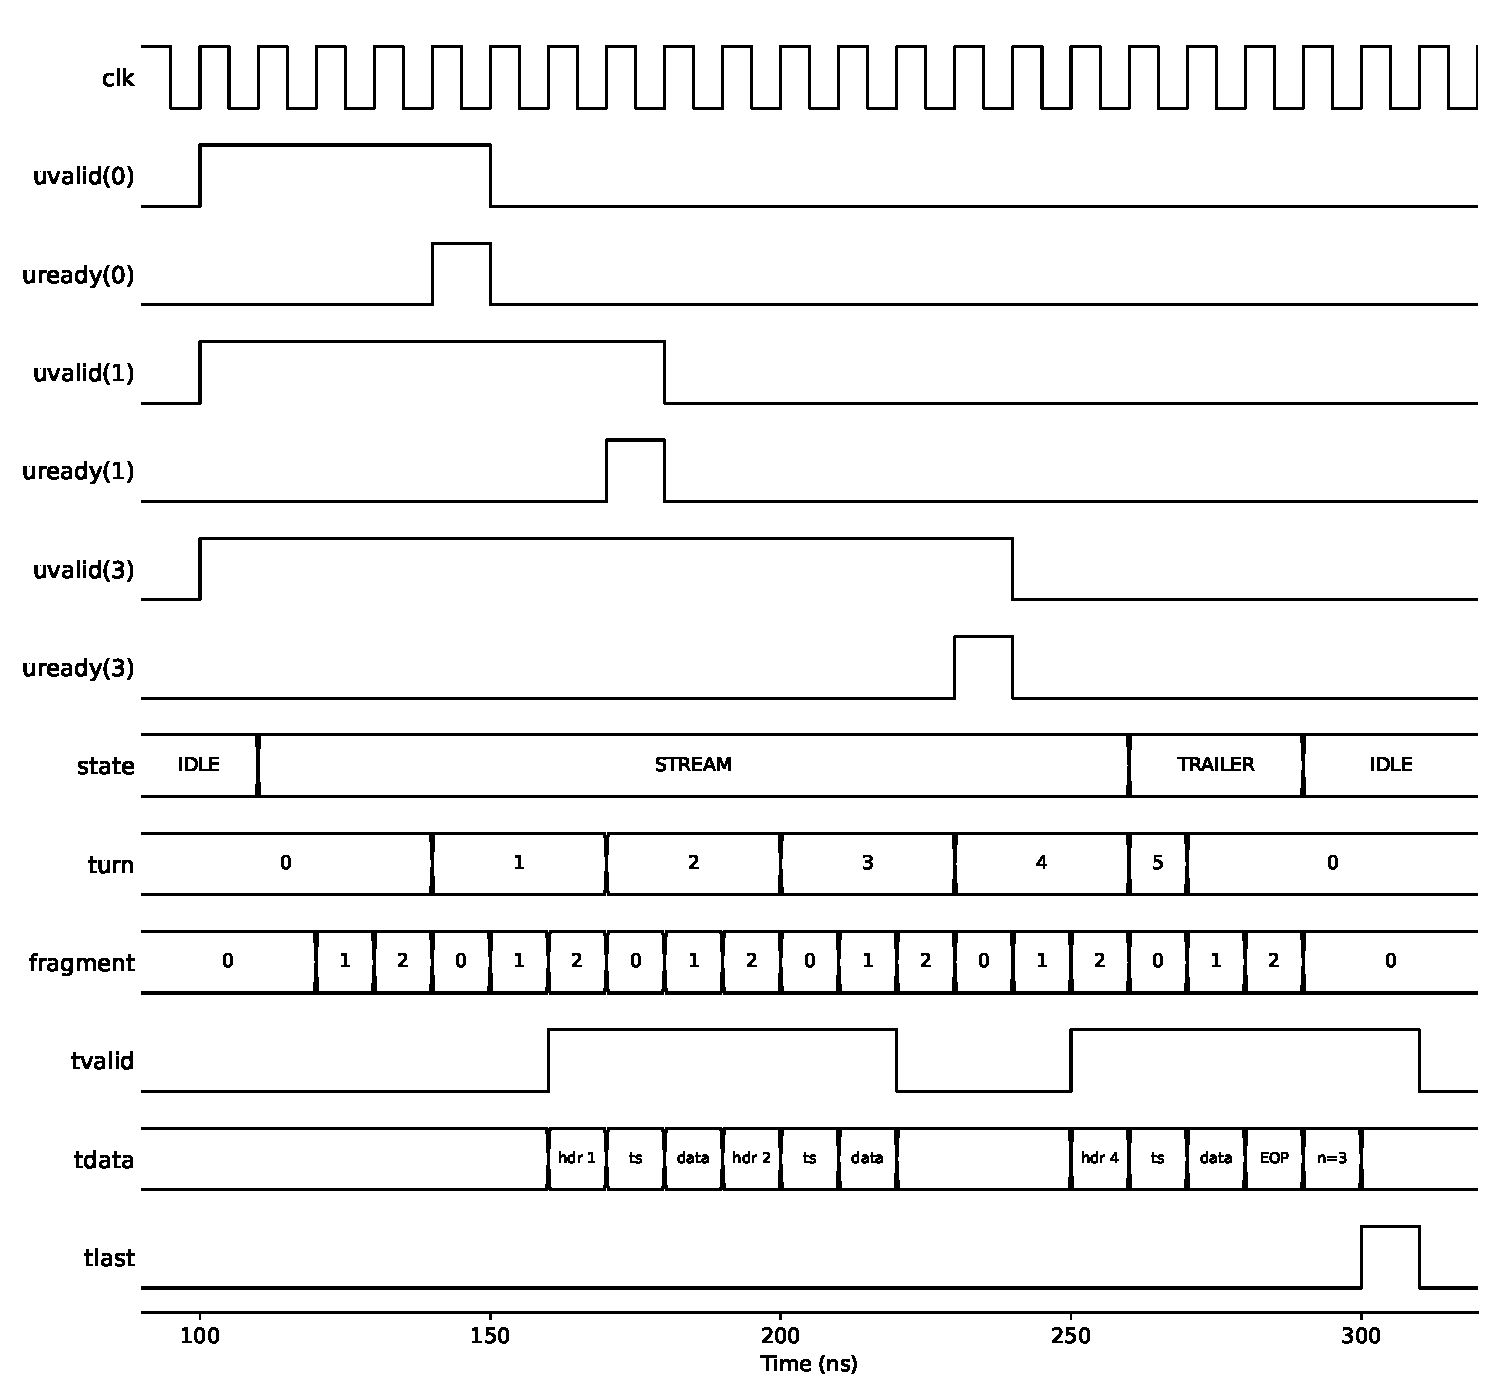
\includegraphics[width=0.9\textwidth]{figs/rx_stream.pdf}
  \caption{\label{fig:rx-stream} The RX buffer streaming three words and the trailer (GHDL simulation of
    {\tt rx\_buffer}; BUFFER\_CONFIG \hex{00030000}: at most 3 words per packet, no timeout).  UARTs 0, 1 and
    3 hold words.  On tdata, ``hdr $n$'' is a header with channel identifier $n$ (UART $n-1$), ``ts'' the
    timestamp, ``data'' the data; the trailer is EOP, the count $n=3$, and a zero fragment with tlast.  Turn
    2 (UART 2, no data) leaves a gap in the stream.  The third word fills the packet, so the trailer follows
    at once.}
\end{figure}

The RX buffer is a state machine with four states: IDLE (no data), STREAM, WAIT (all waiting words sent,
packet still open) and TRAILER.  When any channel has a word waiting, the buffer leaves IDLE and enters
STREAM, starting at turn 0.  Each turn lasts three clock cycles, one per fragment, and visits one channel, in
the order of Table~\ref{tbl:rx-chan}.  In the first clock cycle of a turn the buffer selects the channel; the
multiplexers present that channel's header, timestamp and data; in the third clock cycle, if the channel has
a word waiting, the buffer copies the three fragments and asserts that channel's ready for one clock cycle,
which clears its valid.  The fragments are written to the stream during the following turn.  A channel with
no word costs its three clock cycles, but writes nothing (Fig.~\ref{fig:rx-stream}).  A full sweep of the 44
channels takes 135 clock cycles.  After the sweep, the buffer goes back to WAIT, and from WAIT starts a new
sweep at turn 0 as soon as a word is waiting.  Each sweep therefore starts at UART 0, which keeps the words
of a packet in UART order when the tiles send synchronously.

The stream is closed into DMA packets by the trailer.  BUFFER\_CONFIG sets two conditions, each disabled by
the value zero: a maximum number of words (bits 31--16) and a timeout (bits 15--0, in units of 512 clock
cycles, 5.12\,$\mu$s).  When the packet holds the maximum number of words, the buffer sends the trailer at
the end of the current turn (Fig.~\ref{fig:rx-stream}).  The timeout runs from the first word of the packet,
and is checked only in WAIT, between sweeps: once it has expired, the trailer follows the current sweep.  The
default, \hex{00000001} (no maximum, timeout 512 clock cycles), therefore closes the packet at the end of the
first sweep that ends 512 clock cycles or more after its first word: all the words of one sweep travel in one
packet, and a steady flow of data is cut into packets of about 512 clock cycles.  The trailer's last fragment carries TLAST; the buffer then returns to IDLE.

The buffer never drops data itself.  If the FIFO is full, the stream stalls (tready low), the buffer holds
its current fragments, and the channels keep their words; only a channel that receives a further word before
its word is taken loses data, as counted by UART\_LOST.  The FIFO fill level is available as FIFO\_CNT, and
its maximum since the last clear as FIFO\_MAX.

\subsection{Test pattern}\label{sec:rx-pattern}

The RX unit contains a test pattern generator, which produces a UART stream that any RX channel can receive
in place of its PISO input (INPUT = 4).  When on (PATTERN\_CONFIG bits 11--8 = 1), it repeatedly sends the
64-bit word PATTERN\_B:PATTERN\_A as a UART frame (start bit, 64 bits least significant first, stop bit),
followed by PATTERN\_DELAY bit periods of idle line.  It uses the BAUD strobe for its bit timing, with the
PHASE in PATTERN\_CONFIG bits 7--0, like a TX channel.  All channels set to INPUT = 4 receive the same frames
at the same time, which exercises the whole RX unit, buffer and DMA, at full rate and without any tile.  The
frames sent are counted (PATTERN\_STARTS, PATTERN\_STOPS).

\subsection{RX registers}

\begin{table}[htbp]
\caption{\label{tbl:rx-reg} Registers of the RX unit for each UART (scope \texttt{01}, channel 0--39,
  \hex{00}--\hex{27}).  UART\_CONFIG can also be written at the broadcast channel (\hex{3B}).}
\begin{center}\small
\begin{tabularx}{\textwidth}{llcL}
\toprule
Register          & $R$      & Access & Contents \\
\midrule
UART\_STATUS      & \hex{00} & RO & channel status (Table~\ref{tbl:rx-bits}) \\
UART\_CONFIG      & \hex{04} & RW & Table~\ref{tbl:rx-bits}; default \hex{000A1104} \\
UART\_CHAN        & \hex{08} & RW & channel identifier in the header (bits 15--0); default UART + 1 \\
UART\_STARTS      & \hex{20} & RO & counter: start bits received \\
UART\_BEATS       & \hex{24} & RO & counter: words taken by the RX buffer \\
UART\_UPDATES     & \hex{28} & RO & counter: frames completed (good stop bit) \\
UART\_LOST        & \hex{2C} & RO & counter: words lost (previous word not yet taken) \\
UART\_FRAME\_ERR  & \hex{30} & RO & counter: framing errors (low stop bit) \\
UART\_NOISE       & \hex{34} & RO & counter: sample points with dissenting samples \\
\bottomrule
\end{tabularx}
\end{center}
\end{table}

\begin{table}[htbp]
\caption{\label{tbl:rx-common} Registers of the RX unit in common (scope \texttt{01}, channel \hex{3F}:
  addresses \hex{7F00} + $R$).}
\begin{center}\small
\begin{tabularx}{\textwidth}{llcL}
\toprule
Register          & $R$      & Access & Contents \\
\midrule
PATTERN\_A        & \hex{80} & RW & test pattern word, bits 31--0 \\
PATTERN\_B        & \hex{84} & RW & test pattern word, bits 63--32 \\
PATTERN\_DELAY    & \hex{88} & RW & idle bit periods between test frames \\
PATTERN\_CONFIG   & \hex{8C} & RW & bits 7--0 PHASE, bits 11--8 MODE (1: on) \\
PATTERN\_STATUS   & \hex{90} & RO & bit 0 start, bit 1 stop, bit 8 the pattern line \\
PATTERN\_STARTS   & \hex{94} & RO & counter: test frames started \\
PATTERN\_STOPS    & \hex{98} & RO & counter: test frames completed \\
LOOK\_SELECT      & \hex{A0} & RW & the UART shown by LOOK\_UA and LOOK\_UB \\
LOOK\_UA          & \hex{A4} & RO & that UART's last word, bits 31--0 \\
LOOK\_UB          & \hex{A8} & RO & that UART's last word, bits 63--32 \\
BUFFER\_STATUS    & \hex{B0} & RO & RX buffer status (Table~\ref{tbl:rx-bits}) \\
BUFFER\_CONFIG    & \hex{B4} & RW & bits 31--16 maximum words, bits 15--0 timeout; default \hex{00000001} \\
BUFFER\_ENABLES   & \hex{B8} & RW & extra channels: bit 0 heartbeat, 1 rollover, 2 marker 2, 3 marker 3 \\
PACMAN            & \hex{BC} & RW & PACMAN identifier in the header (bits 7--0) \\
HEARTBEAT\_CONFIG & \hex{C0} & RW & clock cycles between heartbeats; default \hex{3B9ACA00} \\
ROLLOVER\_CONFIG  & \hex{C4} & RW & timestamp (bits 31--0) of the rollover word; default 1 \\
WORD\_TYPE\_LUT   & \hex{C8} & RW & word type for data bits 1--0 = 0, 1, 2, 3 (bytes 0--3); default \hex{44444444} \\
HEADER\_A--D      & \hex{D0}--\hex{DC} & RW & headers of channels 40--43 (Table~\ref{tbl:rx-chan}); bits 15--8 are replaced by the PACMAN identifier in the stream \\
EOP\_HEADER       & \hex{E0} & RW & header of the trailer, bits 15--8 replaced likewise; default \hex{0000004C} \\
FIFO\_CNT         & \hex{F0} & RO & words (64 bits) in the RX FIFO \\
FIFO\_MAX         & \hex{F4} & RO & maximum of FIFO\_CNT since the last clear \\
ZERO\_CNTS        & \hex{F8} & WO & clear all RX counters and FIFO\_MAX (command: any value) \\
\bottomrule
\end{tabularx}
\end{center}
\end{table}

\begin{table}[htbp]
\caption{\label{tbl:rx-bits} Bit fields of the RX registers.}
\begin{center}\small
\begin{tabularx}{\textwidth}{lllL}
\toprule
Register       & Field   & Bits   & Description \\
\midrule
UART\_CONFIG   & PHASE   & 7--0   & MODE 1: clock cycles from the start-bit edge to the sample point; MODE 2: from the BAUD strobe \\
               & INPUT   & 11--8  & one-hot: 0 none (line high), 1 PISO, 2 loopback (POSI), 4 test pattern, 8 emulator (held high in this version) \\
               & MODE    & 13--12 & 0 off, 1 sample point from the start bit, 2 fixed sample point \\
               & FLAGS   & 15--14 & bit 14: accept a start bit with dissenting samples \\
               & PERIOD  & 23--16 & the bit period in clock cycles (equal to the Timing unit's CONFIG\_BAUD) \\
\midrule
UART\_STATUS   & STATE   & 1--0   & 0 idle, 1 start bit, 2 data, 3 stop bit \\
               & HANDSHAKE & 3--2 & ready (bit 3) and valid (bit 2) with the RX buffer \\
               & EVENTS  & 7--4   & frame error, lost, update, start (bits 7--4; one clock cycle each), as counted \\
               & SAMPLING & 11--8 & dissent, sample point, BAUD, noise (bits 11--8) \\
               & TAPS    & 15--12 & majority vote (bit 15) and the three-sample history (bits 14--12) \\
               & INPUTS  & 19--16 & emulator, test pattern, loopback, PISO (bits 19--16) \\
               & EDGE    & 31--24 & edge phase:  position of the last start-bit edge in the bit period \\
\midrule
BUFFER\_STATUS & STATE   & 2--0   & 0 idle, 1 wait, 2 stream, 3 trailer \\
               & STREAM  & 7--3   & stream writer:  last, write, busy, tready, tvalid (bits 7--3) \\
               & TURN    & 13--8  & current turn (channel) \\
               & FRAGMENT & 15--14 & current fragment \\
\bottomrule
\end{tabularx}
\end{center}
\end{table}

The registers of the RX unit are listed in Tables~\ref{tbl:rx-reg} and~\ref{tbl:rx-common}, and their
bit fields in Table~\ref{tbl:rx-bits}.  The counters describe each UART completely: in normal operation STARTS, UPDATES
and BEATS are equal, and LOST, FRAME\_ERR and NOISE are zero.  The look registers show the last word received
by one UART (lost words and words with a framing error excepted).  As in the TX unit, the status registers are snapshots, mainly useful for
debugging.

%======================================================================
\section{Timing unit}\label{sec:atc}

\begin{figure}[htbp]
\centering
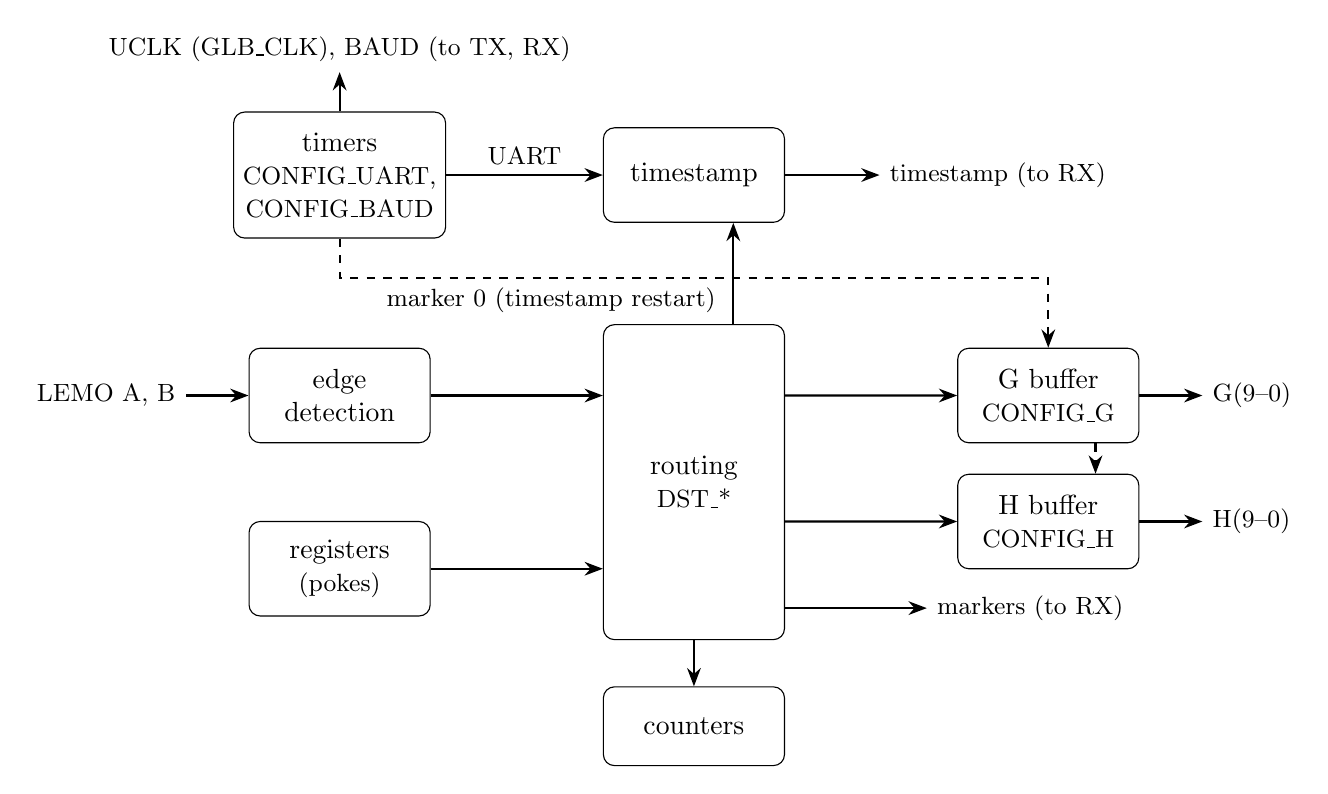
\begin{tikzpicture}[x=1cm, y=1cm, >=Stealth]
\def\bw{2.3cm}
\node[draw, rounded corners, minimum width=\bw, minimum height=1.6cm, align=center] (tim) at (0,6) {timers\\\small CONFIG\_UART,\\\small CONFIG\_BAUD};
\node[draw, rounded corners, minimum width=\bw, minimum height=1.2cm, align=center] (ts) at (4.5,6) {timestamp};
\node[draw, rounded corners, minimum width=\bw, minimum height=1.2cm, align=center] (sync) at (0,3.2) {edge\\detection};
\node[draw, rounded corners, minimum width=\bw, minimum height=1.2cm, align=center] (reg) at (0,1.0) {registers\\\small (pokes)};
\node[draw, rounded corners, minimum width=\bw, minimum height=4.0cm, align=center] (mux) at (4.5,2.1) {routing\\\small DST\_*};
\node[draw, rounded corners, minimum width=\bw, minimum height=1.2cm, align=center] (gb) at (9,3.2) {G buffer\\\small CONFIG\_G};
\node[draw, rounded corners, minimum width=\bw, minimum height=1.2cm, align=center] (hb) at (9,1.6) {H buffer\\\small CONFIG\_H};
\node[draw, rounded corners, minimum width=\bw, minimum height=1.0cm, align=center] (cnt) at (4.5,-1.0) {counters};
\draw[<-, thick] (sync.west) -- ++(-0.8,0) node[anchor=east, font=\small] {LEMO A, B};
\draw[->, thick] (sync.east) -- (mux.west |- sync.east);
\draw[->, thick] (reg.east) -- (mux.west |- reg.east);
\draw[->, thick] (tim.east) -- node[above, font=\small] {UART} (ts.west);
\draw[->, thick] (ts.east) -- ++(1.2,0) node[anchor=west, font=\small] {timestamp (to RX)};
\draw[->, thick] (tim.north) -- ++(0,0.5) node[anchor=south, font=\small] {UCLK (GLB\_CLK), BAUD (to TX, RX)};
\draw[->, thick] ($(mux.east)+(0,1.1)$) -- (gb.west);
\draw[->, thick] ($(mux.east)-(0,0.5)$) -- (hb.west);
\draw[->, thick] ($(mux.north)+(0.5,0)$) -- ++(0,0.9) -| ($(ts.south)+(0.5,0)$);
\node[font=\small, anchor=east] at ($(mux.north)+(0.4,0.3)$) {marker 0 (timestamp restart)};
\draw[->, thick] ($(mux.east)-(0,1.6)$) -- ++(1.8,0) node[anchor=west, font=\small] {markers (to RX)};
\draw[->, thick] (gb.east) -- ++(0.8,0) node[anchor=west, font=\small] {G(9--0)};
\draw[->, thick] (hb.east) -- ++(0.8,0) node[anchor=west, font=\small] {H(9--0)};
\draw[->, thick] (mux.south) -- (cnt.north);
\draw[->, thick, dashed] (tim.south) -- ++(0,-0.5) -| ($(gb.north)$);
\draw[->, thick, dashed] ($(gb.south)+(0.6,0)$) -- ($(hb.north)+(0.6,0)$);
\end{tikzpicture}
\caption{\label{fig:atc-unit} The Timing unit.  The timers set the ASIC clock (UCLK), the UART strobe and the
  BAUD strobe.  The routing sends each stimulus (LEMO inputs, register pokes) to the G and H outputs of
  selected tiles, and to the markers; the G and H buffers align the outputs to the ASIC clock (dashed).  G
  and H are abstract control signals: their meaning on each board is in Table~\ref{tab:atc-gh}.}
\end{figure}

The Timing unit (ATC, for ASIC timing and control, in the firmware sources) produces everything that sets
the time of the system: the ASIC clock, the bit timing of the UARTs, the timestamp, and two control
signals to the ASICs on each tile, G and H.  Its structure is shown in Fig.~\ref{fig:atc-unit}.

G and H are abstract on purpose: the firmware does not name them after a function, because the PACMAN
schematics and the ASIC disagree on what the lines do.  On hw1v5 the line the schematics call SYNC/RST is the
v3 ASIC's reset, and the schematics' TRIG line is the ASIC's SYNC (its trigger function is hardly used).  The
meaning of G and H is set by the board's block design (Table~\ref{tab:atc-gh}).

\begin{table}[H]
\centering
\caption{\label{tab:atc-gh} G and H on each board.}
\begin{tabular}{@{}l>{\raggedright\arraybackslash}p{0.38\linewidth}>{\raggedright\arraybackslash}p{0.38\linewidth}@{}}
\toprule
Board & G & H \\
\midrule
hw1v5 & port SYNC\_O\_0; schematic SYNC/RST; v3 ASIC RST & port TRIG\_O\_0; schematic TRIG; v3 ASIC SYNC (and TRIG) \\
hw1v4 & legacy\_1v4 block, input SYNCN\_I & legacy\_1v4 block, input TRIG\_I \\
\bottomrule
\end{tabular}
\end{table}

\subsection{Clocks and timestamp}

\begin{figure}[htbp]
  \centering
  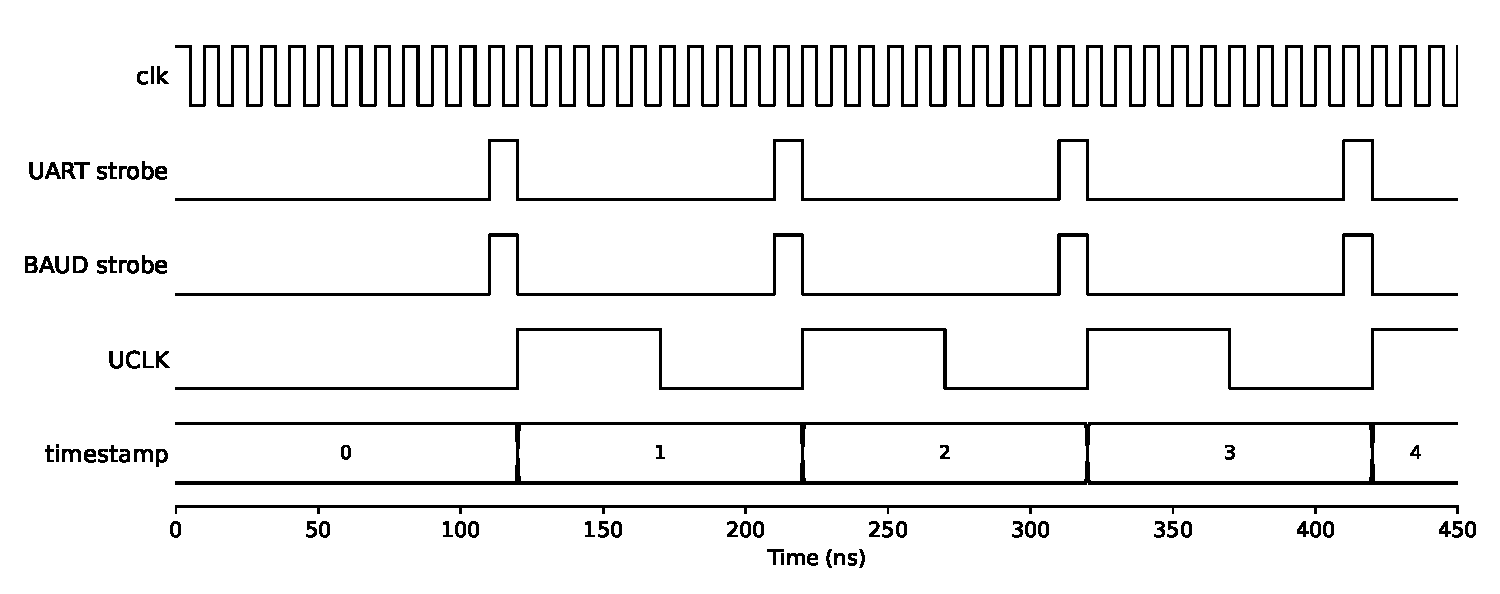
\includegraphics[width=0.9\textwidth]{figs/atc_timer.pdf}
  \caption{\label{fig:atc-timer} The strobes, the ASIC clock and the timestamp after reset (GHDL simulation
    of {\tt atc\_unit}; default periods of 10 clock cycles).  UCLK rises on the clock cycle after each UART
    strobe and falls half a period later; the timestamp counts the UART strobes.}
\end{figure}

Two independent timers count the 100 MHz clock.  The UART timer produces a one-clock strobe every
CONFIG\_UART clock cycles, and the BAUD timer a strobe every CONFIG\_BAUD clock cycles (both 10 by default:
10 MHz).  The UART strobe makes the ASIC clock, UCLK, which is sent to all tiles (GLB\_CLK): it rises after
each UART strobe and falls after half the period, a 50\% duty cycle at the default period.  The BAUD strobe
sets the bit period of all TX and RX channels.  The two are independent, though normally equal.

The timestamp is a 64-bit count of UART strobes, that is, of periods of the ASIC clock
(Fig.~\ref{fig:atc-timer}).  It is attached by the RX unit to every word received, and its least significant
32 bits can be read in the TIMESTAMP register.  Marker 0 restarts the timestamp
(Fig.~\ref{fig:atc-poke}).  Since one stimulus can be routed both to marker 0 and to G or H, the timestamp can
be restarted together with the ASICs (on hw1v5 with the v3 ASIC:  marker 0 and H).

\subsection{Stimuli, routing and outputs}

\begin{figure}[htbp]
  \centering
  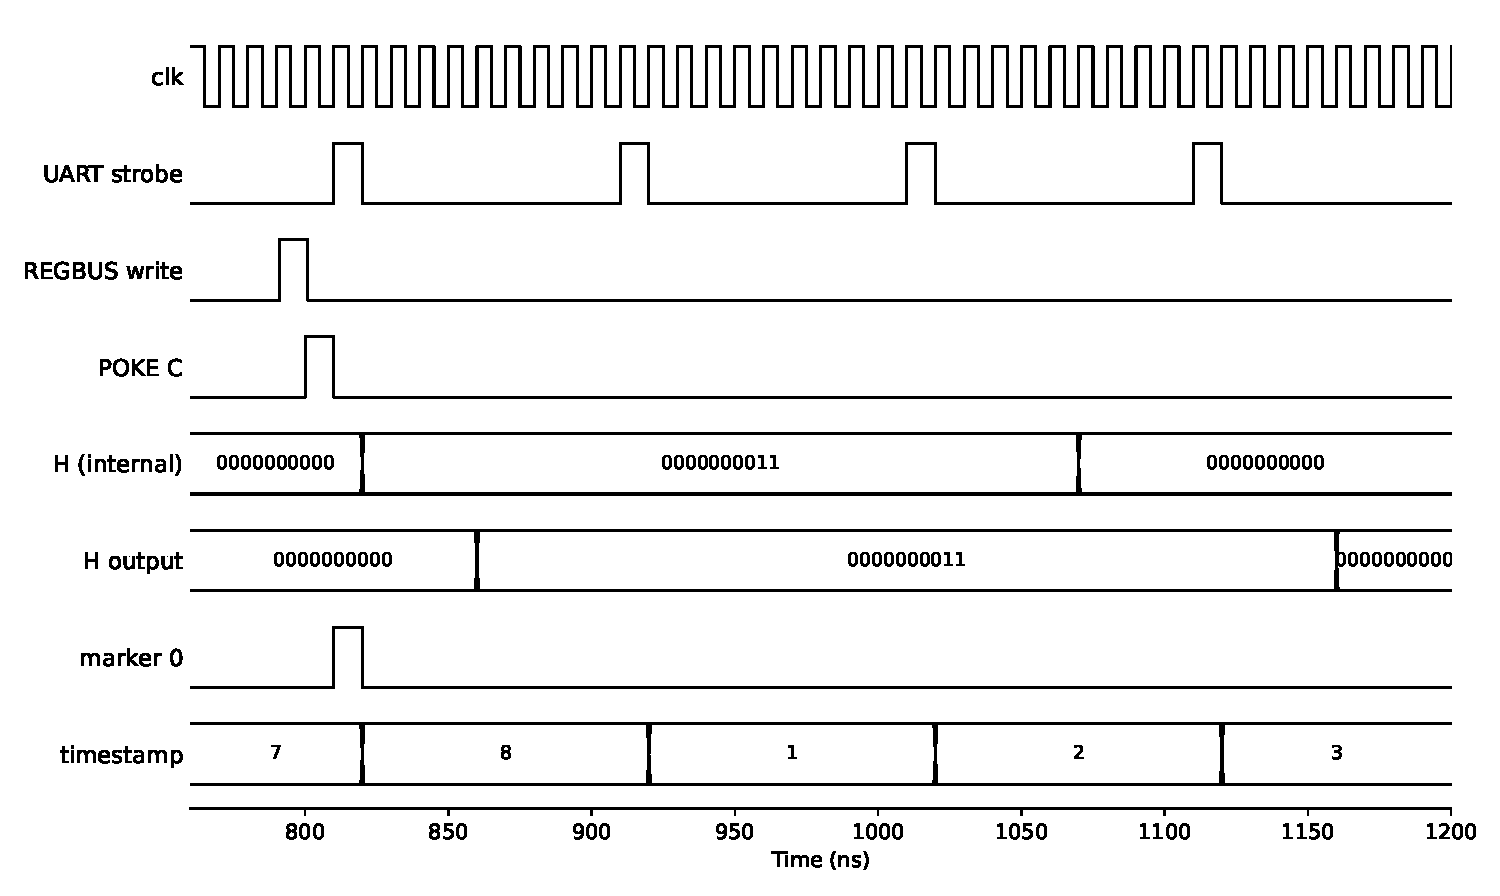
\includegraphics[width=0.9\textwidth]{figs/atc_poke.pdf}
  \caption{\label{fig:atc-poke} A poke routed to H (GHDL simulation of {\tt atc\_unit}).  DST\_POKE\_C is
    \hex{001903C6}: H output, marker 0, tiles 0--3, 25 clock cycles; CONFIG\_H is 3.  The write to POKE\_C
    (\hex{00000003}: tiles 0 and 1) makes a one-clock poke.  The internal H signal is high for 25 clock
    cycles on tiles 0 and 1 only (the destination and the poke's own mask); the output is aligned to the UART
    strobe plus 3 clock cycles, and so lasts three UART periods.  Marker 0 restarts the timestamp.}
\end{figure}

Each signal that the Timing unit can send to the tiles starts as a {\em stimulus}, a one-clock pulse.  There
are eight stimuli: the two front-panel LEMO inputs (A and B), four {\em pokes} (A to D), made by writing to the
POKE\_A to POKE\_D registers, and two internal sources (LOGIC A and B), which are disabled in this version.
Each stimulus has a destination register (DST\_LEMO\_A to DST\_LOGIC\_B, Table~\ref{tbl:atc-dst}), which
says where it goes and for how long: to the G outputs, the H outputs, or both, on the tiles of its tile mask,
for a duration of a set number of clock cycles; and to any of the four markers, as a one-clock pulse.  A
stimulus with a destination of zero goes nowhere, which is the default.

\begin{table}[htbp]
\caption{\label{tbl:atc-dst} Bit fields of the destination registers DST\_LEMO\_A to DST\_LOGIC\_B.}
\begin{center}
\begin{tabularx}{\textwidth}{llL}
\toprule
Field    & Bits    & Description \\
\midrule
G        & 0       & send to the G outputs \\
H        & 1       & send to the H outputs \\
MARKERS  & 5--2    & send to markers 0--3 (one clock cycle) \\
TILES    & 15--6   & tile mask for G and H: bit 6 for tile 0, \ldots, bit 15 for tile 9 \\
DURATION & 31--16  & length of the G and H pulse, in clock cycles \\
\bottomrule
\end{tabularx}
\end{center}
\end{table}

A poke carries a further tile mask of its own, in bits 9--0 of the value written to POKE\_A to POKE\_D: the
pulse reaches a tile only if both the destination and the poke select it.  The PS can therefore pulse any set
of tiles with a single write, without changing the destination.  A new stimulus restarts the duration of its
own pulse; pulses of different stimuli on the same output are combined.

The G and H signals of each tile pass an output buffer before they leave the PL.  The buffer samples
its input once per UART period, at a point set by PHASE (CONFIG\_G and CONFIG\_H bits 7--0, in clock cycles
after the UART strobe), and holds its output until the next sample, so that G and H change at a fixed
point of the ASIC clock and last a whole number of ASIC clock periods.  A pulse shorter than one UART period
may fall between two samples and be missed: the DURATION of a destination with G or H should be at least the
UART period (10 clock cycles by default).  The buffer can also invert the signal of each tile (bits 17--8, one
per tile); an inverted output is high when idle.  Figure~\ref{fig:atc-poke} shows a poke on its way through the unit.

\begin{figure}[htbp]
  \centering
  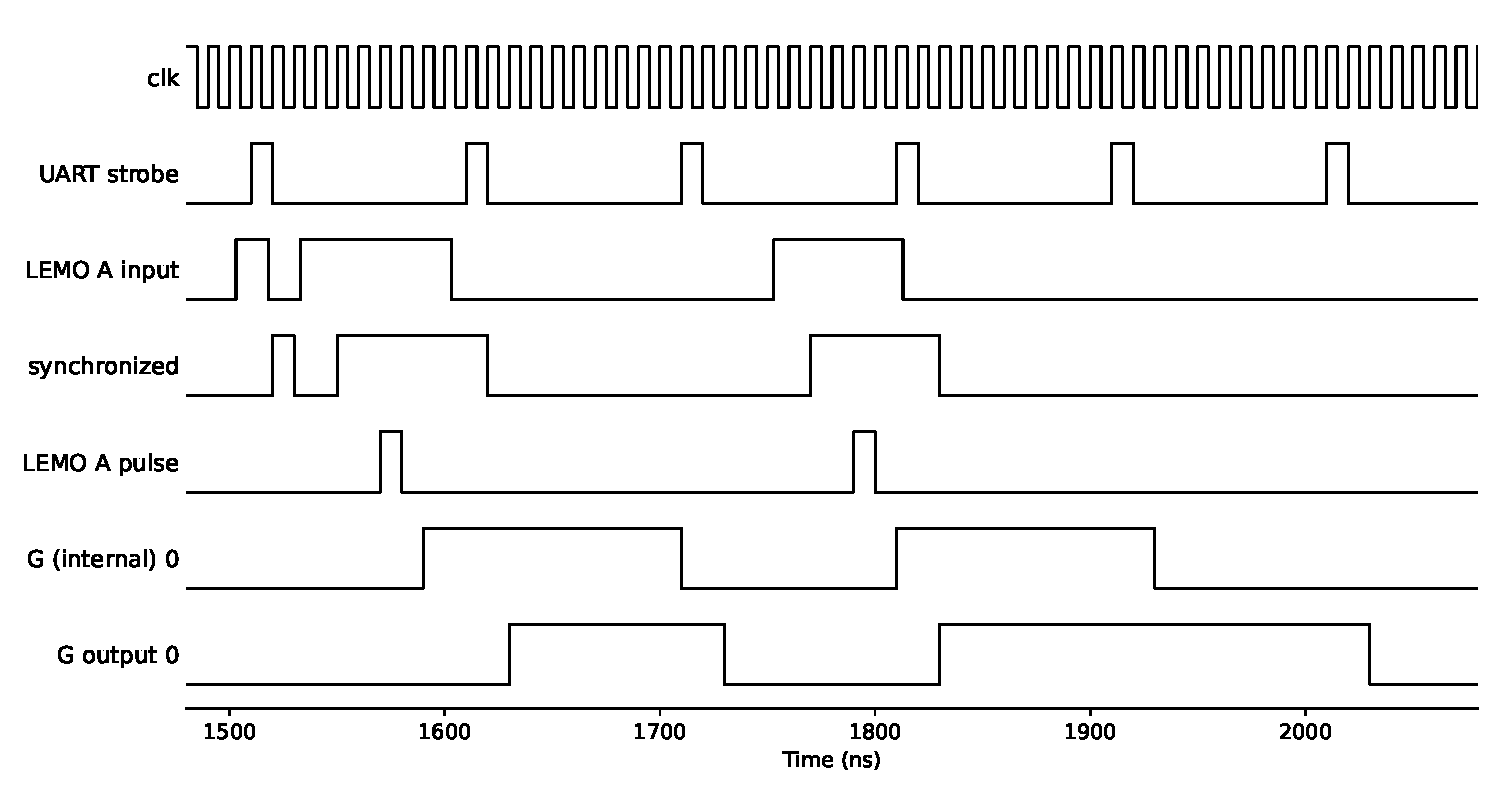
\includegraphics[width=0.9\textwidth]{figs/atc_lemo.pdf}
  \caption{\label{fig:atc-lemo} A LEMO input routed to G (GHDL simulation of {\tt atc\_unit}; DST\_LEMO\_A
    \hex{000CFFC1}: G output, all tiles, 12 clock cycles; CONFIG\_G 0).  The first high, 15\,ns long, is
    seen by the synchronizer for one clock cycle only, which is not an edge.  Each rising edge after it
    makes one pulse, which is routed to G for 12 clock cycles and aligned to the UART strobe.}
\end{figure}

The LEMO inputs are asynchronous.  Each passes a two-stage synchronizer, and a rising edge is detected when
the synchronized input is high on two consecutive clock cycles after being low; no further edge is detected
during the next few clock cycles.  A pulse must therefore be seen high on two clock cycles: one shorter than
10\,ns is always ignored, and one shorter than 20\,ns may be (Fig.~\ref{fig:atc-lemo}).
CONFIG\_INPUT bits 0 and 1 invert LEMO A and B, so that a falling edge is detected instead.

The markers connect the Timing unit to the data.  Marker 0 restarts the timestamp.  Markers 2 and 3
are channels 42 and 43 of the RX buffer: when enabled there, each marker pulse adds a word with its
timestamp to the stream.  A LEMO trigger input routed to marker 2, for example, records the time of every
external trigger along with the data.  Marker 1 is only counted.

\subsection{Counters}

\begin{table}[htbp]
\caption{\label{tbl:atc-cmd} Commands of the counters, written to COUNT\_REQ (bits 7--0).}
\begin{center}
\begin{tabularx}{\textwidth}{llL}
\toprule
Command & Code (bits 7--4) & Description (bits 3--0: the channel $C$) \\
\midrule
NO OP   & 0 & nothing \\
CLEAR   & 1 & clear all counters \\
START   & 2 & start all counters (the default after reset) \\
STOP    & 3 & stop all counters \\
READ M  & 4 & latch the counter of marker $C$ (0--3) into COUNT \\
READ G  & 5 & latch the counter of the G signal of tile $C$ (0--9) \\
READ H  & 6 & latch the counter of the H signal of tile $C$ (0--9) \\
READ I  & 7 & latch the counter of stimulus $C$: 0 LEMO A, 1 LEMO B, 2--5 POKE A--D \\
\bottomrule
\end{tabularx}
\end{center}
\end{table}

The Timing unit counts its signals: the stimuli (LEMO and pokes), the G and H signals of each tile (before
the output buffers), and the markers.  Each counter holds two 16-bit numbers, both saturating: the number of
rising edges, and the {\em integral}, the number of clock cycles during which the signal was high (counted only
after its first rising edge since the counters were cleared).  The counters are controlled by commands written to COUNT\_REQ
(Table~\ref{tbl:atc-cmd}).  A READ command latches one counter into the COUNT register, as integral
(bits 31--16) and edges (bits 15--0), where it can then be read.  The counters run from reset; STOP, START and
CLEAR act on all of them together.

\subsection{Timing registers}

\begin{table}[htbp]
\caption{\label{tbl:atc-reg} Registers of the Timing unit (scope \texttt{1110}).}
\begin{center}\small
\begin{tabularx}{\textwidth}{llcL}
\toprule
Register        & Address     & Access & Contents \\
\midrule
STATUS          & \hex{E000} & RO & zero (no status bits defined) \\
TIMESTAMP       & \hex{E004} & RO & timestamp, bits 31--0 \\
POKE\_A--D      & \hex{E0A0}, \hex{E0B0}, \hex{E0C0}, \hex{E0D0} & WO & poke (command); bits 9--0: the poke's tile mask \\
CONFIG\_UART    & \hex{E100} & RW & UART (and UCLK) period in clock cycles; default 10 \\
CONFIG\_BAUD    & \hex{E104} & RW & bit period of the TX and RX channels in clock cycles; default 10 \\
CONFIG\_INPUT   & \hex{E108} & RW & bit 0: invert LEMO A, bit 1: invert LEMO B \\
CONFIG\_G       & \hex{E110} & RW & G output buffer: bits 7--0 PHASE, bits 17--8 invert (per tile) \\
CONFIG\_H       & \hex{E114} & RW & H output buffer: bits 7--0 PHASE, bits 17--8 invert (per tile) \\
DST\_LEMO\_A, \_B & \hex{E120}, \hex{E124} & RW & destination of LEMO A, B (Table~\ref{tbl:atc-dst}) \\
DST\_POKE\_A--D & \hex{E128}--\hex{E134} & RW & destination of POKE A--D \\
DST\_LOGIC\_A, \_B & \hex{E138}, \hex{E13C} & RW & destination of LOGIC A, B (disabled sources) \\
COUNT\_REQ      & \hex{E200} & WO & counter command (Table~\ref{tbl:atc-cmd}) \\
COUNT           & \hex{E204} & RO & latched counter: bits 31--16 integral, bits 15--0 edges \\
\bottomrule
\end{tabularx}
\end{center}
\end{table}

The registers of the Timing unit are listed in Table~\ref{tbl:atc-reg}.  All configuration registers are
zero after reset, except the two periods.  The Timing unit answers reads and writes on the next clock cycle,
like the Global unit.

\end{document}
